\chapter{Applications}
\label{chp:applications}
%You are free to write up any additional material that will appear in the final
%report, for example a section or chapter describing a significant component of
%the design/implementation that you have already completed.  Avoid any
%additional material that is not re-usable in the final report.

\newcommand{\gscaling}{0.7}

\newcommand{\gone}{
    \begin{tabular}{>{\centering\bfseries}m{1in} >{\centering}m{0in}}	
      \begin{tikzpicture}[scale=\gscaling,auto,swap]

	% define the round nodes
	\foreach \pos/\name/\label in {
	  {(0,1)//1a},
	  {(0,0)//2a},
	  {(0,-1)//3a}}
	  \node[vertex2] (\label) at \pos {$\name$} ;

	%neighbouring graph
	      
	\path[hi, line width=1.0]  (1a)  -- (2a);
	\path[hi, line width=1.0]  (2a)  -- (3a);

	
      \end{tikzpicture} & \Large{$G_{1}$}
    \end{tabular}
}

\newcommand{\gonecca}[1]{
    \begin{tabular}{>{\centering\bfseries}m{0.4in} >{\centering}m{0in}}	
      \begin{tikzpicture}[scale=\gscaling,auto,swap]

	% define the round nodes
	\foreach \pos/\name/\label in {
	  {(0,1)//1a},
	  {(0,0)//2a},
	  {(0,-1)//3a}}
	  \node[vertex2,draw=#1,fill=#1] (\label) at \pos {$\name$} ;

	%neighbouring graph
	      
	\path[hi, line width=1.0,draw=#1]  (1a)  -- (2a);
	\path[hi, line width=1.0,draw=#1]  (2a)  -- (3a);

	
      \end{tikzpicture} \cellcolor{black} & \cellcolor{black}\textcolor{white}{\Large{$G_{1}$}}
    \end{tabular}
}

\newcommand{\gtwo}{
    \begin{tabular}{>{\centering\bfseries}m{1in} >{\centering}m{0in}}	
      \begin{tikzpicture}[scale=\gscaling * 1.3,auto,swap]

	% define the round nodes
	\foreach \pos/\name/\label in {
	  {(0,1.3)//1a},
	  {(-0.7,0)//2a},
	  {(0.7,0)//3a}}
	  \node[vertex2] (\label) at \pos {$\name$} ;

	%neighbouring graph
	      
	\path[hi, line width=1.0]  (1a)  -- (2a);
	\path[hi, line width=1.0]  (2a)  -- (3a);
	\path[hi, line width=1.0]  (3a)  -- (1a);

	
      \end{tikzpicture} & \Large{$G_{2}$}
    \end{tabular}
}


\newcommand{\gtwocca}[1]{
    \begin{tabular}{>{\centering\bfseries}m{0.7in} >{\centering}m{0in}}	
      \begin{tikzpicture}[scale=\gscaling * 1.3,auto,swap]

	% define the round nodes
	\foreach \pos/\name/\label in {
	  {(0,1.3)//1a},
	  {(-0.7,0)//2a},
	  {(0.7,0)//3a}}
	  \node[vertex3,draw=#1,fill=#1] (\label) at \pos {$\name$} ;

	%neighbouring graph
	      
	\path[hi, line width=1.0,draw=#1]  (1a)  -- (2a);
	\path[hi, line width=1.0,draw=#1]  (2a)  -- (3a);
	\path[hi, line width=1.0,draw=#1]  (3a)  -- (1a);

	
      \end{tikzpicture} \cellcolor{black} & \cellcolor{black}\textcolor{white}{\Large{$G_{2}$}}
    \end{tabular}
}

\newcommand{\gfive}{
    \begin{tabular}{>{\centering\bfseries}m{1in} >{\centering}m{0in}}	
      \begin{tikzpicture}[scale=\gscaling * 1.5,auto,swap]

	% define the round nodes
	\foreach \pos/\name/\label in {
	  {(0,0)//1a},
	  {(0,1)//2a},
	  {(1,1)//3a},
	  {(1,0)//4a}}
	  \node[vertex2] (\label) at \pos {$\name$} ;

	%neighbouring graph
	      
	\path[hi, line width=1.0]  (1a)  -- (2a);
	\path[hi, line width=1.0]  (2a)  -- (3a);
	\path[hi, line width=1.0]  (3a)  -- (4a);
	\path[hi, line width=1.0]  (1a)  -- (4a);


	
      \end{tikzpicture} & \Large{$G_{5}$}
    \end{tabular}
}

\newcommand{\gsix}{
    \begin{tabular}{>{\centering\bfseries}m{1in} >{\centering}m{0in}}	
      \begin{tikzpicture}[scale=\gscaling,auto,swap]

	% define the round nodes
	\foreach \pos/\name/\label in {
	  {(0,0)//1a},
	  {(-0.8,1)//2a},
	  {(0.8,1)//3a},
	  {(0,-1)//4a}}
	  \node[vertex2] (\label) at \pos {$\name$} ;

	%neighbouring graph
	      
	\path[hi, line width=1.0]  (1a)  -- (2a);
	\path[hi, line width=1.0]  (2a)  -- (3a);
	\path[hi, line width=1.0]  (1a)  -- (3a);
	\path[hi, line width=1.0]  (1a)  -- (4a);


	
      \end{tikzpicture} & \Large{$G_{6}$}
    \end{tabular}
}


\newcommand{\gsixcca}[1]{
    \begin{tabular}{>{\centering\bfseries}m{0.7in} >{\centering}m{0in}}	
      \begin{tikzpicture}[scale=\gscaling,auto,swap]

	% define the round nodes
	\foreach \pos/\name/\label in {
	  {(0,0)//1a},
	  {(-0.8,1)//2a},
	  {(0.8,1)//3a},
	  {(0,-1)//4a}}
	  \node[vertex2,draw=#1,fill=#1] (\label) at \pos {$\name$} ;

	%neighbouring graph
	      
	\path[hi, line width=1.0,draw=#1]  (1a)  -- (2a);
	\path[hi, line width=1.0,draw=#1]  (2a)  -- (3a);
	\path[hi, line width=1.0,draw=#1]  (1a)  -- (3a);
	\path[hi, line width=1.0,draw=#1]  (1a)  -- (4a);


	
      \end{tikzpicture} \cellcolor{black} & \cellcolor{black}\textcolor{white}{\Large{$G_{6}$}}
    \end{tabular}
}

\newcommand{\gseven}{
    \begin{tabular}{>{\centering\bfseries}m{1in} >{\centering}m{0in}}	
      \begin{tikzpicture}[scale=\gscaling * 1.2,auto,swap]

	% define the round nodes
	\foreach \pos/\name/\label in {
	  {(-1.0,0)//1a},
	  {(1,0)//2a},
	  {(0,1)//3a},
	  {(0,-1)//4a}}
	  \node[vertex2] (\label) at \pos {$\name$} ;

	%neighbouring graph
	      
	\path[hi, line width=1.0]  (1a)  -- (3a);
	\path[hi, line width=1.0]  (1a)  -- (4a);
	\path[hi, line width=1.0]  (2a)  -- (3a);
	\path[hi, line width=1.0]  (2a)  -- (4a);
	\path[hi, line width=1.0]  (3a)  -- (4a);

	
      \end{tikzpicture} & \Large{$G_{7}$}
    \end{tabular}
}


\newcommand{\geight}{
    \begin{tabular}{>{\centering\bfseries}m{1in} >{\centering}m{0in}}	
      \begin{tikzpicture}[scale=\gscaling * 1.3,auto,swap]

	% define the round nodes
	\foreach \pos/\name/\label in {
	  {(0,0)//1a},
	  {(-0.7,-0.6)//2a},
	  {(0.7,-0.6)//3a},
	  {(0,1)//4a}}
	  \node[vertex2] (\label) at \pos {$\name$} ;

	%neighbouring graph
	      
	\path[hi, line width=1.0]  (1a)  -- (2a);
	\path[hi, line width=1.0]  (1a)  -- (3a);
	\path[hi, line width=1.0]  (1a)  -- (4a);
	\path[hi, line width=1.0]  (2a)  -- (3a);
	\path[hi, line width=1.0]  (2a)  -- (4a);
	\path[hi, line width=1.0]  (3a)  -- (4a);

	
      \end{tikzpicture} & \Large{$G_{8}$}
    \end{tabular}
}



\newcommand{\geightcca}[1]{
    \begin{tabular}{>{\centering\bfseries}m{0.7in} >{\centering}m{0in}}	
      \begin{tikzpicture}[scale=\gscaling * 1.3,auto,swap]

	% define the round nodes
	\foreach \pos/\name/\label in {
	  {(0,0)//1a},
	  {(-0.7,-0.6)//2a},
	  {(0.7,-0.6)//3a},
	  {(0,1)//4a}}
	  \node[vertex3,draw=#1,fill=#1] (\label) at \pos {$\name$} ;

	%neighbouring graph
	      
	\path[hi, line width=1.0,draw=#1]  (1a)  -- (2a);
	\path[hi, line width=1.0,draw=#1]  (1a)  -- (3a);
	\path[hi, line width=1.0,draw=#1]  (1a)  -- (4a);
	\path[hi, line width=1.0,draw=#1]  (2a)  -- (3a);
	\path[hi, line width=1.0,draw=#1]  (2a)  -- (4a);
	\path[hi, line width=1.0,draw=#1]  (3a)  -- (4a);

	
      \end{tikzpicture} \cellcolor{black} & \cellcolor{black}\textcolor{white}{\Large{$G_{8}$}}
    \end{tabular}
}

\newcommand{\gnine}{
    \begin{tabular}{>{\centering\bfseries}m{1in} >{\centering}m{0in}}	
      \begin{tikzpicture}[scale=\gscaling,auto,swap]

	% define the round nodes
	\foreach \pos/\name/\label in {
	  {(0,2)//1a},
	  {(0,1)//2a},
	  {(0,0)//3a},
	  {(0,-1)//4a},
	  {(0,-2)//5a}}
	  \node[vertex2] (\label) at \pos {$\name$} ;

	%neighbouring graph
	      
	\path[hi, line width=1.0]  (1a)  -- (2a);
	\path[hi, line width=1.0]  (2a)  -- (3a);
	\path[hi, line width=1.0]  (3a)  -- (4a);
	\path[hi, line width=1.0]  (4a)  -- (5a);


	
      \end{tikzpicture} & \Large{$G_{9}$}
    \end{tabular}
}

\newcommand{\gninecca}[1]{
    \begin{tabular}{>{\centering\bfseries}m{0.7in} >{\centering}m{0in}}	
      \begin{tikzpicture}[scale=\gscaling,auto,swap]

	% define the round nodes
	\foreach \pos/\name/\label in {
	  {(0,2)//1a},
	  {(0,1)//2a},
	  {(0,0)//3a},
	  {(0,-1)//4a},
	  {(0,-2)//5a}}
	  \node[vertex3,draw=#1,fill=#1] (\label) at \pos {$\name$} ;

	%neighbouring graph
	      
	\path[hi, line width=1.0,draw=#1]  (1a)  -- (2a);
	\path[hi, line width=1.0,draw=#1]  (2a)  -- (3a);
	\path[hi, line width=1.0,draw=#1]  (3a)  -- (4a);
	\path[hi, line width=1.0,draw=#1]  (4a)  -- (5a);


	
      \end{tikzpicture} \cellcolor{black} & \cellcolor{black}\textcolor{white}{\Large{$G_{9}$}}
    \end{tabular}
}


\newcommand{\gten}{
    \begin{tabular}{>{\centering\bfseries}m{1in} >{\centering}m{0in}}	
      \begin{tikzpicture}[scale=\gscaling,auto,swap]

	% define the round nodes
	\foreach \pos/\name/\label in {
	  {(0,2)//1a},
	  {(0,1)//2a},
	  {(0,0)//3a},
	  {(-0.7,-0.7)//4a},
	  {(0.7,-0.7)//5a}}
	  \node[vertex2] (\label) at \pos {$\name$} ;

	%neighbouring graph
	      
	\path[hi, line width=1.0]  (1a)  -- (2a);
	\path[hi, line width=1.0]  (2a)  -- (3a);
	\path[hi, line width=1.0]  (3a)  -- (4a);
	\path[hi, line width=1.0]  (3a)  -- (5a);


	
      \end{tikzpicture} & \Large{$G_{10}$}
    \end{tabular}
}



\newcommand{\gtencca}[1]{
    \begin{tabular}{>{\centering\bfseries}m{0.7in} >{\centering}m{0in}}	
      \begin{tikzpicture}[scale=\gscaling,auto,swap]

	% define the round nodes
	\foreach \pos/\name/\label in {
	  {(0,2)//1a},
	  {(0,1)//2a},
	  {(0,0)//3a},
	  {(-0.7,-0.7)//4a},
	  {(0.7,-0.7)//5a}}
	  \node[vertex3,draw=#1,fill=#1] (\label) at \pos {$\name$} ;

	%neighbouring graph
	      
	\path[hi, line width=1.0,draw=#1]  (1a)  -- (2a);
	\path[hi, line width=1.0,draw=#1]  (2a)  -- (3a);
	\path[hi, line width=1.0,draw=#1]  (3a)  -- (4a);
	\path[hi, line width=1.0,draw=#1]  (3a)  -- (5a);


	
      \end{tikzpicture} \cellcolor{black} & \cellcolor{black}\textcolor{white}{\Large{$G_{10}$}}
    \end{tabular}
}

\newcommand{\geleven}{
    \begin{tabular}{>{\centering\bfseries}m{1in} >{\centering}m{0in}}	
      \begin{tikzpicture}[scale=\gscaling,auto,swap]

	% define the round nodes
	\foreach \pos/\name/\label in {
	  {(0,0)//1a},
	  {(0,1)//2a},
	  {(-1,0)//3a},
	  {(0,-1)//4a},
	  {(1,0)//5a}}
	  \node[vertex2] (\label) at \pos {$\name$} ;

	%neighbouring graph
	      
	\path[hi, line width=1.0]  (1a)  -- (2a);
	\path[hi, line width=1.0]  (1a)  -- (3a);
	\path[hi, line width=1.0]  (1a)  -- (4a);
	\path[hi, line width=1.0]  (1a)  -- (5a);


	
      \end{tikzpicture} & \Large{$G_{11}$}
    \end{tabular}
}


\newcommand{\gtwelve}{
    \begin{tabular}{>{\centering\bfseries}m{1in} >{\centering}m{0in}}	
      \begin{tikzpicture}[scale=\gscaling,auto,swap]

	% define the round nodes
	\foreach \pos/\name/\label in {
	  {(-0.7,0)//1a},
	  {(0.7,0)//2a},
	  {(0,1.2)//3a},
	  {(-0.7,-1)//4a},
	  {(0.7,-1)//5a}}
	  \node[vertex2] (\label) at \pos {$\name$} ;

	%neighbouring graph
	      
	\path[hi, line width=1.0]  (1a)  -- (2a);
	\path[hi, line width=1.0]  (2a)  -- (3a);
	\path[hi, line width=1.0]  (1a)  -- (3a);
	\path[hi, line width=1.0]  (1a)  -- (4a);
	\path[hi, line width=1.0]  (2a)  -- (5a);

	
      \end{tikzpicture} & \Large{$G_{12}$}
    \end{tabular}
}

\newcommand{\gtwelvecca}[1]{
    \begin{tabular}{>{\centering\bfseries}m{0.7in} >{\centering}m{0in}}	
      \begin{tikzpicture}[scale=\gscaling,auto,swap]

	% define the round nodes
	\foreach \pos/\name/\label in {
	  {(-0.7,0)//1a},
	  {(0.7,0)//2a},
	  {(0,1.2)//3a},
	  {(-0.7,-1)//4a},
	  {(0.7,-1)//5a}}
	  \node[vertex3,draw=#1,fill=#1] (\label) at \pos {$\name$} ;

	%neighbouring graph
	      
	\path[hi, line width=1.0,draw=#1]  (1a)  -- (2a);
	\path[hi, line width=1.0,draw=#1]  (2a)  -- (3a);
	\path[hi, line width=1.0,draw=#1]  (1a)  -- (3a);
	\path[hi, line width=1.0,draw=#1]  (1a)  -- (4a);
	\path[hi, line width=1.0,draw=#1]  (2a)  -- (5a);

	
      \end{tikzpicture}\cellcolor{black} & \cellcolor{black}\textcolor{white}{\Large{$G_{12}$}}
    \end{tabular}
}

\newcommand{\gthirteen}{
    \begin{tabular}{>{\centering\bfseries}m{1in} >{\centering}m{0in}}	
      \begin{tikzpicture}[scale=\gscaling,auto,swap]

	% define the round nodes
	\foreach \pos/\name/\label in {
	  {(0,0)//1a},
	  {(-0.8,1)//2a},
	  {(0.8,1)//3a},
	  {(0,-1)//4a},
	  {(0,-2)//5a}}
	  \node[vertex2] (\label) at \pos {$\name$} ;

	%neighbouring graph
	      
	\path[hi, line width=1.0]  (1a)  -- (2a);
	\path[hi, line width=1.0]  (2a)  -- (3a);
	\path[hi, line width=1.0]  (1a)  -- (3a);
	\path[hi, line width=1.0]  (1a)  -- (4a);
	\path[hi, line width=1.0]  (4a)  -- (5a);

	
      \end{tikzpicture} & \Large{$G_{13}$}
    \end{tabular}
}

\newcommand{\gthirteencca}[1]{
    \begin{tabular}{>{\centering\bfseries}m{0.7in} >{\centering}m{0in}}	
      \begin{tikzpicture}[scale=\gscaling,auto,swap]

	% define the round nodes
	\foreach \pos/\name/\label in {
	  {(0,0)//1a},
	  {(-0.8,1)//2a},
	  {(0.8,1)//3a},
	  {(0,-1)//4a},
	  {(0,-2)//5a}}
	  \node[vertex3,draw=#1,fill=#1] (\label) at \pos {$\name$} ;

	%neighbouring graph
	      
	\path[hi, line width=1.0,draw=#1]  (1a)  -- (2a);
	\path[hi, line width=1.0,draw=#1]  (2a)  -- (3a);
	\path[hi, line width=1.0,draw=#1]  (1a)  -- (3a);
	\path[hi, line width=1.0,draw=#1]  (1a)  -- (4a);
	\path[hi, line width=1.0,draw=#1]  (4a)  -- (5a);

	
      \end{tikzpicture} \cellcolor{black} & \cellcolor{black}\textcolor{white}{\Large{$G_{13}$}}
    \end{tabular}
}


\newcommand{\gfourteen}{
    \begin{tabular}{>{\centering\bfseries}m{1in} >{\centering}m{0in}}	
      \begin{tikzpicture}[scale=\gscaling * 0.8,auto,swap]

	% define the round nodes
	\foreach \pos/\name/\label in {
	  {(0,0)//1a},
	  {(-1,1)//2a},
	  {(1,1)//3a},
	  {(-1,-1)//4a},
	  {(1,-1)//5a}}
	  \node[vertex2] (\label) at \pos {$\name$} ;

	%neighbouring graph
	      
	\path[hi, line width=1.0]  (1a)  -- (2a);
	\path[hi, line width=1.0]  (1a)  -- (3a);
	\path[hi, line width=1.0]  (2a)  -- (3a);
	\path[hi, line width=1.0]  (1a)  -- (4a);
	\path[hi, line width=1.0]  (1a)  -- (5a);

	
      \end{tikzpicture} & \Large{$G_{14}$}
    \end{tabular}
}



\newcommand{\gfourteencca}[1]{
    \begin{tabular}{>{\centering\bfseries}m{0.7in} >{\centering}m{0in}}	
      \begin{tikzpicture}[scale=\gscaling * 0.8,auto,swap]

	% define the round nodes
	\foreach \pos/\name/\label in {
	  {(0,0)//1a},
	  {(-1,1)//2a},
	  {(1,1)//3a},
	  {(-1,-1)//4a},
	  {(1,-1)//5a}}
	  \node[vertex3,draw=#1,fill=#1] (\label) at \pos {$\name$} ;

	%neighbouring graph
	      
	\path[hi, line width=1.0,draw=#1]  (1a)  -- (2a);
	\path[hi, line width=1.0,draw=#1]  (1a)  -- (3a);
	\path[hi, line width=1.0,draw=#1]  (2a)  -- (3a);
	\path[hi, line width=1.0,draw=#1]  (1a)  -- (4a);
	\path[hi, line width=1.0,draw=#1]  (1a)  -- (5a);

	
      \end{tikzpicture} \cellcolor{black} & \cellcolor{black}\textcolor{white}{\Large{$G_{14}$}}
    \end{tabular}
}

\newcommand{\gfifteen}{
    \begin{tabular}{>{\centering\bfseries}m{1in} >{\centering}m{0in}}	
      \begin{tikzpicture}[scale=\gscaling,auto,swap]

	% define the round nodes
	\foreach \pos/\name/\label in {
	  {(0,1)//1a},
	  {(-0.8,0.2)//2a},
	  {(-0.4,-0.8)//3a},
	  {(0.4,-0.8)//4a},
	  {(0.8,0.2)//5a}}
	  \node[vertex2] (\label) at \pos {$\name$} ;

	%neighbouring graph
	      
	\path[hi, line width=1.0]  (1a)  -- (2a);
	\path[hi, line width=1.0]  (2a)  -- (3a);
	\path[hi, line width=1.0]  (3a)  -- (4a);
	\path[hi, line width=1.0]  (4a)  -- (5a);
	\path[hi, line width=1.0]  (5a)  -- (1a);

	
      \end{tikzpicture} & \Large{$G_{15}$}
    \end{tabular}
}

\newcommand{\gfifteencca}[1]{
    \begin{tabular}{>{\centering\bfseries}m{0.7in} >{\centering}m{0in}}	
      \begin{tikzpicture}[scale=\gscaling,auto,swap]

	% define the round nodes
	\foreach \pos/\name/\label in {
	  {(0,1)//1a},
	  {(-0.8,0.2)//2a},
	  {(-0.4,-0.8)//3a},
	  {(0.4,-0.8)//4a},
	  {(0.8,0.2)//5a}}
	  \node[vertex2,draw=#1,fill=#1] (\label) at \pos {$\name$} ;

	%neighbouring graph
	      
	\path[hi, line width=1.0,draw=#1]  (1a)  -- (2a);
	\path[hi, line width=1.0,draw=#1]  (2a)  -- (3a);
	\path[hi, line width=1.0,draw=#1]  (3a)  -- (4a);
	\path[hi, line width=1.0,draw=#1]  (4a)  -- (5a);
	\path[hi, line width=1.0,draw=#1]  (5a)  -- (1a);

	
      \end{tikzpicture} \cellcolor{black} & \cellcolor{black}\textcolor{white}{\Large{$G_{15}$}}
    \end{tabular}
}


\newcommand{\gsixteen}{
    \begin{tabular}{>{\centering\bfseries}m{1in} >{\centering}m{0in}}	
      \begin{tikzpicture}[scale=\gscaling,auto,swap]

	% define the round nodes
	\foreach \pos/\name/\label in {
	  {(0,0)//1a},
	  {(-0.8,1)//2a},
	  {(0.8,1)//3a},
	  {(0,-1)//4a},
	  {(0,1.8)//5a}}
	  \node[vertex2] (\label) at \pos {$\name$} ;

	%neighbouring graph
	      
	\path[hi, line width=1.0]  (1a)  -- (2a);
	\path[hi, line width=1.0]  (2a)  -- (5a);
	\path[hi, line width=1.0]  (3a)  -- (5a);
	\path[hi, line width=1.0]  (1a)  -- (3a);
	\path[hi, line width=1.0]  (1a)  -- (4a);


      \end{tikzpicture} & \Large{$G_{16}$}
    \end{tabular}
}



\newcommand{\gsixteencca}[1]{
    \begin{tabular}{>{\centering\bfseries}m{0.7in} >{\centering}m{0in}}	
      \begin{tikzpicture}[scale=\gscaling,auto,swap]

	% define the round nodes
	\foreach \pos/\name/\label in {
	  {(0,0)//1a},
	  {(-0.8,1)//2a},
	  {(0.8,1)//3a},
	  {(0,-1)//4a},
	  {(0,1.8)//5a}}
	  \node[vertex3,draw=#1,fill=#1] (\label) at \pos {$\name$} ;

	%neighbouring graph
	      
	\path[hi, line width=1.0,draw=#1]  (1a)  -- (2a);
	\path[hi, line width=1.0,draw=#1]  (2a)  -- (5a);
	\path[hi, line width=1.0,draw=#1]  (3a)  -- (5a);
	\path[hi, line width=1.0,draw=#1]  (1a)  -- (3a);
	\path[hi, line width=1.0,draw=#1]  (1a)  -- (4a);


      \end{tikzpicture} \cellcolor{black} & \cellcolor{black}\textcolor{white}{\Large{$G_{16}$}}
    \end{tabular}
}

\newcommand{\gtwenty}{
    \begin{tabular}{>{\centering\bfseries}m{1in} >{\centering}m{0in}}	
      \begin{tikzpicture}[scale=\gscaling,auto,swap]

	% define the round nodes
	\foreach \pos/\name/\label in {
	  {(-1.0,0)//1a},
	  {(0,0)//2a},
	  {(1,0)//3a},
	  {(0,1)//4a},
	  {(0,-1)//5a}}
	  \node[vertex2] (\label) at \pos {$\name$} ;

	%neighbouring graph
	      
	\path[hi, line width=1.0]  (1a)  -- (4a);
	\path[hi, line width=1.0]  (2a)  -- (4a);
	\path[hi, line width=1.0]  (3a)  -- (4a);
	\path[hi, line width=1.0]  (1a)  -- (5a);
	\path[hi, line width=1.0]  (2a)  -- (5a);
	\path[hi, line width=1.0]  (3a)  -- (5a);

	
      \end{tikzpicture} & \Large{$G_{20}$}
    \end{tabular}
}

\newcommand{\gtwentycca}[1]{
    \begin{tabular}{>{\centering\bfseries}m{0.7in} >{\centering}m{0in}}	
      \begin{tikzpicture}[scale=\gscaling,auto,swap]

	% define the round nodes
	\foreach \pos/\name/\label in {
	  {(-1.0,0)//1a},
	  {(0,0)//2a},
	  {(1,0)//3a},
	  {(0,1)//4a},
	  {(0,-1)//5a}}
	  \node[vertex2,draw=#1,fill=#1] (\label) at \pos {$\name$} ;

	%neighbouring graph
	      
	\path[hi, line width=1.0,draw=#1]  (1a)  -- (4a);
	\path[hi, line width=1.0,draw=#1]  (2a)  -- (4a);
	\path[hi, line width=1.0,draw=#1]  (3a)  -- (4a);
	\path[hi, line width=1.0,draw=#1]  (1a)  -- (5a);
	\path[hi, line width=1.0,draw=#1]  (2a)  -- (5a);
	\path[hi, line width=1.0,draw=#1]  (3a)  -- (5a);

	
      \end{tikzpicture} \cellcolor{black} & \cellcolor{black}\textcolor{white}{\Large{$G_{20}$}}
    \end{tabular}
}


\newcommand{\gtwentyone}{
    \begin{tabular}{>{\centering\bfseries}m{1in} >{\centering}m{0in}}	
      \begin{tikzpicture}[scale=\gscaling * 1.4,auto,swap]

	% define the round nodes
	\foreach \pos/\name/\label in {
	  {(0,0)//1a},
	  {(1,0)//2a},
	  {(0.5,0.7)//3a},
	  {(0,-1)//4a},
	  {(1,-1)//5a}}
	  \node[vertex2] (\label) at \pos {$\name$} ;

	%neighbouring graph
	      
	\path[hi, line width=1.0]  (1a)  -- (2a);
	\path[hi, line width=1.0]  (1a)  -- (3a);
	\path[hi, line width=1.0]  (2a)  -- (3a);
	\path[hi, line width=1.0]  (1a)  -- (4a);
	\path[hi, line width=1.0]  (2a)  -- (5a);
	\path[hi, line width=1.0]  (4a)  -- (5a);

	
      \end{tikzpicture} & \Large{$G_{21}$}
    \end{tabular}
}


\newcommand{\gtwentytwo}{
    \begin{tabular}{>{\centering\bfseries}m{1in} >{\centering}m{0in}}	
      \begin{tikzpicture}[scale=\gscaling * 1.4,auto,swap]

	% define the round nodes
	\foreach \pos/\name/\label in {
	  {(0,0)//1a},
	  {(1,0)//2a},
	  {(0.5,0.7)//3a},
	  {(0.5,-0.7)//4a},
	  {(0.5,-1.6)//5a}}
	  \node[vertex2] (\label) at \pos {$\name$} ;

	%neighbouring graph

	\path[hi, line width=1.0]  (1a)  -- (2a);	
	\path[hi, line width=1.0]  (1a)  -- (3a);
	\path[hi, line width=1.0]  (1a)  -- (4a);
	\path[hi, line width=1.0]  (1a)  -- (5a);
	\path[hi, line width=1.0]  (2a)  -- (3a);
	\path[hi, line width=1.0]  (2a)  -- (4a);
	\path[hi, line width=1.0]  (2a)  -- (5a);

	
      \end{tikzpicture} & \Large{$G_{22}$}
    \end{tabular}
}


\newcommand{\gtwentythree}{
    \begin{tabular}{>{\centering\bfseries}m{1in} >{\centering}m{0in}}	
      \begin{tikzpicture}[scale=\gscaling * 1.2,auto,swap]

	% define the round nodes
	\foreach \pos/\name/\label in {
	  {(0,0)//1a},
	  {(-0.7,-0.6)//2a},
	  {(0.7,-0.6)//3a},
	  {(0,1)//4a},
	  {(-0.7,-1.6)//5a}}
	  \node[vertex2] (\label) at \pos {$\name$} ;

	%neighbouring graph
	      
	\path[hi, line width=1.0]  (1a)  -- (2a);
	\path[hi, line width=1.0]  (1a)  -- (3a);
	\path[hi, line width=1.0]  (1a)  -- (4a);
	\path[hi, line width=1.0]  (2a)  -- (3a);
	\path[hi, line width=1.0]  (2a)  -- (4a);
	\path[hi, line width=1.0]  (3a)  -- (4a);
	\path[hi, line width=1.0]  (2a)  -- (5a);
	
      \end{tikzpicture} & \Large{$G_{23}$}
    \end{tabular}
}


\newcommand{\gtwentyfour}{
    \begin{tabular}{>{\centering\bfseries}m{1in} >{\centering}m{0in}}	
      \begin{tikzpicture}[scale=\gscaling * 1.3,auto,swap]

	% define the round nodes
	\foreach \pos/\name/\label in {
	  {(0,0)//1a},
	  {(0,1)//2a},
	  {(0.8,0.6)//3a},
	  {(0.8,-0.6)//4a},
	  {(0,-1)//5a}}
	  \node[vertex2] (\label) at \pos {$\name$} ;

	%neighbouring graph

	\path[hi, line width=1.0]  (1a)  -- (2a);	
	\path[hi, line width=1.0]  (1a)  -- (3a);
	\path[hi, line width=1.0]  (1a)  -- (4a);
	\path[hi, line width=1.0]  (1a)  -- (5a);
	\path[hi, line width=1.0]  (2a)  -- (3a);
	\path[hi, line width=1.0]  (3a)  -- (4a);
	\path[hi, line width=1.0]  (4a)  -- (5a);

	
      \end{tikzpicture} & \Large{$G_{24}$}
    \end{tabular}
}


\newcommand{\gtwentyfive}{
    \begin{tabular}{>{\centering\bfseries}m{1in} >{\centering}m{0in}}	
      \begin{tikzpicture}[scale=\gscaling * 1.2,auto,swap]

	% define the round nodes
	\foreach \pos/\name/\label in {
	  {(-1.0,0)//1a},
	  {(0,0)//2a},
	  {(1,0)//3a},
	  {(0,1)//4a},
	  {(0,-1)//5a}}
	  \node[vertex2] (\label) at \pos {$\name$} ;

	%neighbouring graph

	\path[hi, line width=1.0]  (1a)  -- (2a);	
	\path[hi, line width=1.0]  (1a)  -- (4a);
	\path[hi, line width=1.0]  (2a)  -- (4a);
	\path[hi, line width=1.0]  (3a)  -- (4a);
	\path[hi, line width=1.0]  (1a)  -- (5a);
	\path[hi, line width=1.0]  (2a)  -- (5a);
	\path[hi, line width=1.0]  (3a)  -- (5a);

	
      \end{tikzpicture} & \Large{$G_{25}$}
    \end{tabular}
}


\newcommand{\gtwentysix}{
    \begin{tabular}{>{\centering\bfseries}m{1in} >{\centering}m{0in}}	
      \begin{tikzpicture}[scale=\gscaling * 1.0,auto,swap]

	% define the round nodes
	\foreach \pos/\name/\label in {
	  {(-0.8,0)//1a},
	  {(0.8,0)//2a},
	  {(0,0.75)//3a},
	  {(0,-0.75)//4a},
	  {(0,-1.8)//5a}}
	  \node[vertex2] (\label) at \pos {$\name$} ;

	%neighbouring graph

	\path[hi, line width=1.0]  (1a)  -- (2a);	
	\path[hi, line width=1.0]  (1a)  -- (3a);
	\path[hi, line width=1.0]  (1a)  -- (4a);
	\path[hi, line width=1.0]  (1a)  -- (5a);
	\path[hi, line width=1.0]  (2a)  -- (3a);
	\path[hi, line width=1.0]  (2a)  -- (4a);
	\path[hi, line width=1.0]  (2a)  -- (5a);

	
      \end{tikzpicture} & \Large{$G_{26}$}
    \end{tabular}
}



\newcommand{\gtwentyseven}{
    \begin{tabular}{>{\centering\bfseries}m{1in} >{\centering}m{0in}}	
      \begin{tikzpicture}[scale=\gscaling*2,auto,swap]

	% define the round nodes
	\foreach \pos/\name/\label in {
	  {(0,0)//1a},
	  {(0,1)//2a},
	  {(1,1)//3a},
	  {(1,0)//4a},
	  {(0.5,0.5)//5a}}
	  \node[vertex2] (\label) at \pos {$\name$} ;

	%neighbouring graph
	      
	\path[hi, line width=1.0]  (1a)  -- (2a);
	\path[hi, line width=1.0]  (2a)  -- (3a);
	\path[hi, line width=1.0]  (3a)  -- (4a);
	\path[hi, line width=1.0]  (1a)  -- (4a);
	\path[hi, line width=1.0]  (5a)  -- (2a);
	\path[hi, line width=1.0]  (5a)  -- (3a);
	\path[hi, line width=1.0]  (5a)  -- (4a);
	\path[hi, line width=1.0]  (5a)  -- (1a);

	
      \end{tikzpicture} & \Large{$G_{27}$}
    \end{tabular}
}


\newcommand{\gtwentynine}{
    \begin{tabular}{>{\centering\bfseries}m{1in} >{\centering}m{0in}}	
      \begin{tikzpicture}[scale=\gscaling * 1.3,auto,swap]

	% define the round nodes
	\foreach \pos/\name/\label in {
	  {(0,1)//1a},
	  {(-0.8,0.2)//2a},
	  {(-0.4,-0.8)//3a},
	  {(0.4,-0.8)//4a},
	  {(0.8,0.2)//5a}}
	  \node[vertex2] (\label) at \pos {$\name$} ;

	%neighbouring graph
	      
	\path[hi, line width=1.0]  (1a)  -- (2a);
	\path[hi, line width=1.0]  (1a)  -- (3a);
	\path[hi, line width=1.0]  (1a)  -- (4a);
	\path[hi, line width=1.0]  (1a)  -- (5a);
	\path[hi, line width=1.0]  (2a)  -- (3a);
	\path[hi, line width=1.0]  (2a)  -- (4a);
	\path[hi, line width=1.0]  (2a)  -- (5a);
	\path[hi, line width=1.0]  (3a)  -- (4a);
	\path[hi, line width=1.0]  (3a)  -- (5a);
	\path[hi, line width=1.0]  (4a)  -- (5a);


	
      \end{tikzpicture} & \Large{$G_{29}$}
    \end{tabular}
}

\newcommand{\gtwentyninecca}[1]{
    \begin{tabular}{>{\centering\bfseries}m{0.7in} >{\centering}m{0in}}	
      \cellcolor{black}\begin{tikzpicture}[scale=\gscaling * 1.3,auto,swap]

	% define the round nodes
	\foreach \pos/\name/\label in {
	  {(0,1)//1a},
	  {(-0.8,0.2)//2a},
	  {(-0.4,-0.8)//3a},
	  {(0.4,-0.8)//4a},
	  {(0.8,0.2)//5a}}
	  \node[vertex3,draw=#1,fill=#1] (\label) at \pos {$\name$} ;

	%neighbouring graph
	      
	\path[hi, line width=1.0,draw=#1]  (1a)  -- (2a);
	\path[hi, line width=1.0,draw=#1]  (1a)  -- (3a);
	\path[hi, line width=1.0,draw=#1]  (1a)  -- (4a);
	\path[hi, line width=1.0,draw=#1]  (1a)  -- (5a);
	\path[hi, line width=1.0,draw=#1]  (2a)  -- (3a);
	\path[hi, line width=1.0,draw=#1]  (2a)  -- (4a);
	\path[hi, line width=1.0,draw=#1]  (2a)  -- (5a);
	\path[hi, line width=1.0,draw=#1]  (3a)  -- (4a);
	\path[hi, line width=1.0,draw=#1]  (3a)  -- (5a);
	\path[hi, line width=1.0,draw=#1]  (4a)  -- (5a);


	
      \end{tikzpicture} & \cellcolor{black}\textcolor{white}{\Large{$G_{29}$}}
    \end{tabular}
}


\newcommand{\gdots}{
    \begin{tabular}{>{\centering\bfseries}m{-2in} >{\centering}m{0in}}	
    \vdots & 
    \end{tabular}
}


\definecolor{ccacol0}{rgb}{0.00,1.00,0}%1
\definecolor{ccacol1}{rgb}{0.20,1.00,0}%0.8 
\definecolor{ccacol2}{rgb}{0.40,1.00,0}%0.6
\definecolor{ccacol3}{rgb}{0.60,1.00,0}%0.4
\definecolor{ccacol4}{rgb}{0.80,1.00,0}%0.2
\definecolor{ccacol5}{rgb}{1.00,1.00,0}%0.0
\definecolor{ccacol6}{rgb}{1.00,0.80,0}%-0.2
\definecolor{ccacol7}{rgb}{1.00,0.60,0}%-0.4
\definecolor{ccacol8}{rgb}{1.00,0.40,0}%-0.6
\definecolor{ccacol9}{rgb}{1.00,0.20,0}%-0.8
\definecolor{ccacol10}{rgb}{1.00,0.00,0}%-1


\newcommand{\ccafigscale}{0.75}



\section{Initial Experiments}



\subsection{Average Network GCV}

The first experiments we conduct with the novel GCV signature are comparisons of average network GCV signatures. For each node in the given network, the normalised GCV signature is calculated and then averaged over all the nodes in the network. Figure \ref{fig:avg_gdv_real} shows the results for three different networks: A Human PPI network, a Human Metabolic network and a 2010 World Trade network. 


\begin{figure}[h]
  \centering
  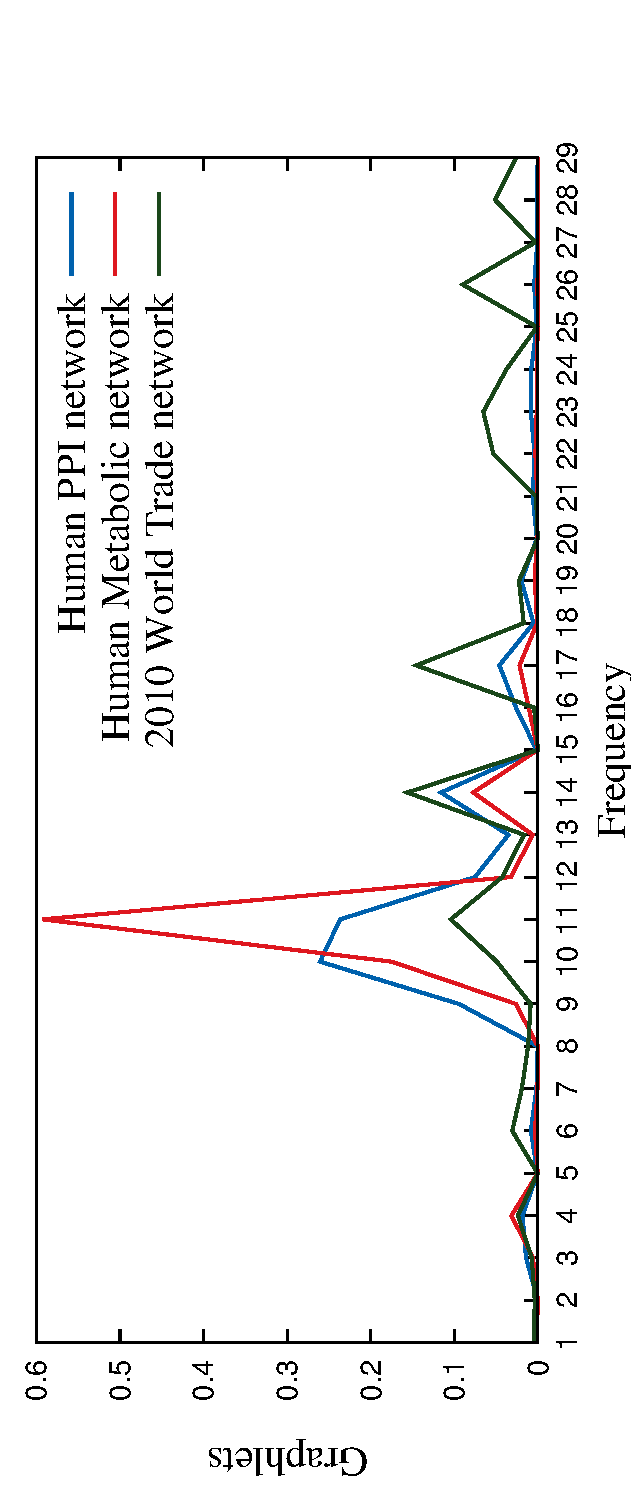
\includegraphics[scale=0.7, angle=-90]{../code/final_results/all_nets_average2.pdf}
  \caption[Average GCV signatures for PPI, Metabolic and World Trade network]{Comparison of the average GCV signatures for three different
  real networks: a PPI network, a Metabolic network and 
  a 2010 World Trade network (WTN). There is a considerable discrepancy in the values of graphlets \{9,10,11\} across the network types. Moreover, the WTN is the only network in which graphlets \{22,23,24,26,28,29\} are represented.}
  \label{fig:avg_gdv_real}
\end{figure}

We observe in figure \ref{fig:avg_gdv_real} that there are slight differences between the normalised GCV of the three networks analysed. More precisely,
Graphlets \{9,10,11\} seem to discriminate well between them, with the Metabolic network having the highest number of $ G_{11}$ graphlets and the WTN having the least. All these graphlets are sparse 5-node graphlets that have 4 edges each. The reason why the Metabolic network has a lot of graphlets $G_{11}$ (a claw of 5 nodes) is because it is made of long metabolic paths that intersect with each other. This is best represented by graphlet $G_{11}$ which is made of a central node and several satellite nodes. Moreover, the WTN also seems to have relatively more graphlets \{22,26,28,29,22,23,24\} compared to the other networks. The reason for this is because the WTN is a dense network and all those graphlets are relatively dense compared to graphlets \{9,10,11, \dots \} that have few connecting edges.

\subsection{Random Networks}
\label{sec:initial_experiments_rnd_nets}

After we performed comparisons of the average GCV of real networks, our
next step is to experiment with the following random network models:
\begin{enumerate}
  \item Erd\H{o}s-R\'{e}nyi \cite{erdHos1959random} (ER)
  \item Erd\H{o}s-R\'{e}nyi (with preserved\footnote{The "stubs" method enables the Erd\H{o}s-R\'{e}nyi graph to preserve the degree distribution of the real network.} degree distribution) (ER-DD)
  \item Geometric networks \cite{penrose2003random} (GEO)
  \item Scale-free Barab\'{a}si-Albert -- preferential attachment \cite{barabasi1999emergence} (SF)
  \item Stickiness index-based \cite{prvzulj2006modelling} (STICKY)
\end{enumerate}


The corresponding labels (ER, ER-DD, GEO, SF, STICKY) will be used throughout this section to refer to each of these models. We generate 30 different models for every network (Metabolic, PPI, WTN) and random network generating algorithm (ER, ER-DD, etc ..) resulting in 150 total networks. Afterwards, in order to give a measure of precision to the GCV signature of random networks, we calculate the standard deviation for each of the values of the GCV. 

The results obtained for the Human PPI network are shown in figure \ref{ppi_spreads}. For the Human PPI network, we notice that all the random models apart from ER-DD have very low standard deviations for all the graphlet frequencies. The graphlets where the ER-DD networks exhibit some degree of randomness are \{10, 11\}. On the other hand, the geometric random graphs are the only ones which contain some of the dense 5-node graphlets at the right-end of the spectrum \{23,24,26,28,29\}. Moreover, the ER random graphs only contain graphlet $G_1$, which is a $P3$. The reason for this is because ER is a rudimentary random graph model that is unable to capture the underlying complexity of the original graph. The random networks that seem to best approximate the original networks are the Scale-free\footnote{Barab\'{a}si-Albert Preferential Attachment} and the Stickiness-based. These results are confirmed by the \emph{Relative Cluster Frequency Agreement} in section \ref{rcfd_res}.


\begin{figure}[H]
  \centering
  \textbf{Average GCV for random models of the Human PPI network}
  \begin{subfigure}[b]{1.0\textwidth}
    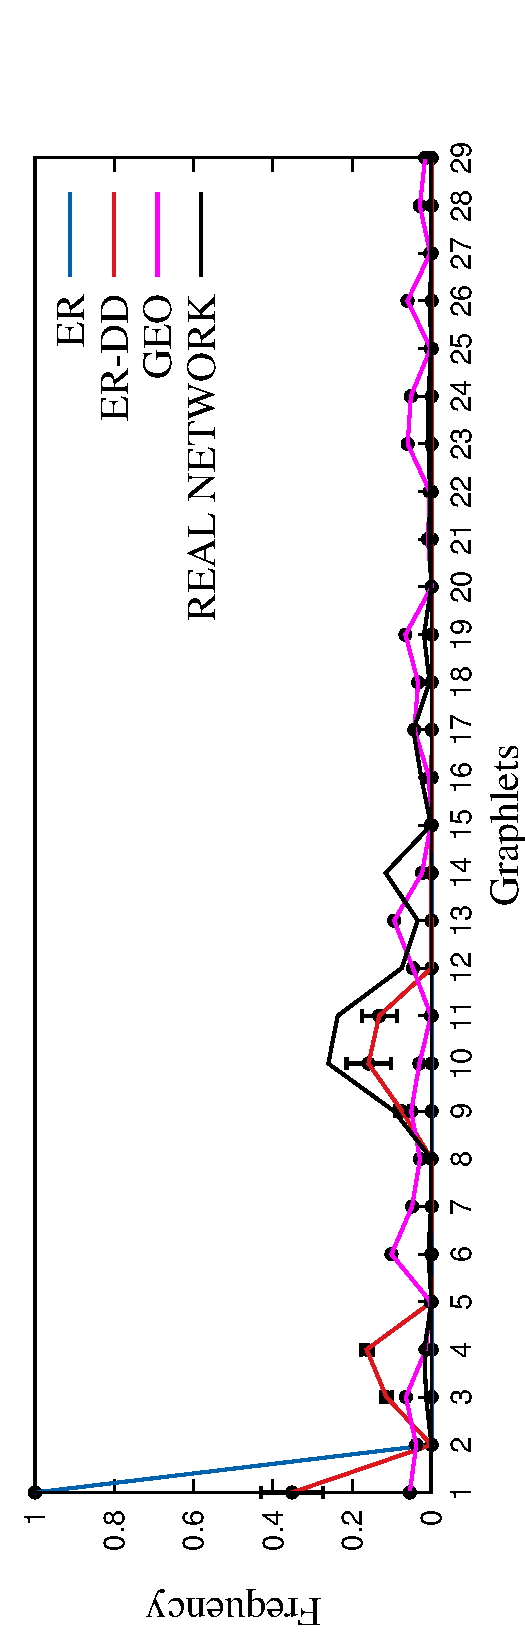
\includegraphics[angle=-90,scale=0.6]{../code/final_results/human_ppi/avg_egdvs_rnd_spreads_figures/spreads_012_rnd2.pdf} 
  \end{subfigure}
  \begin{subfigure}[b]{1.0\textwidth}
    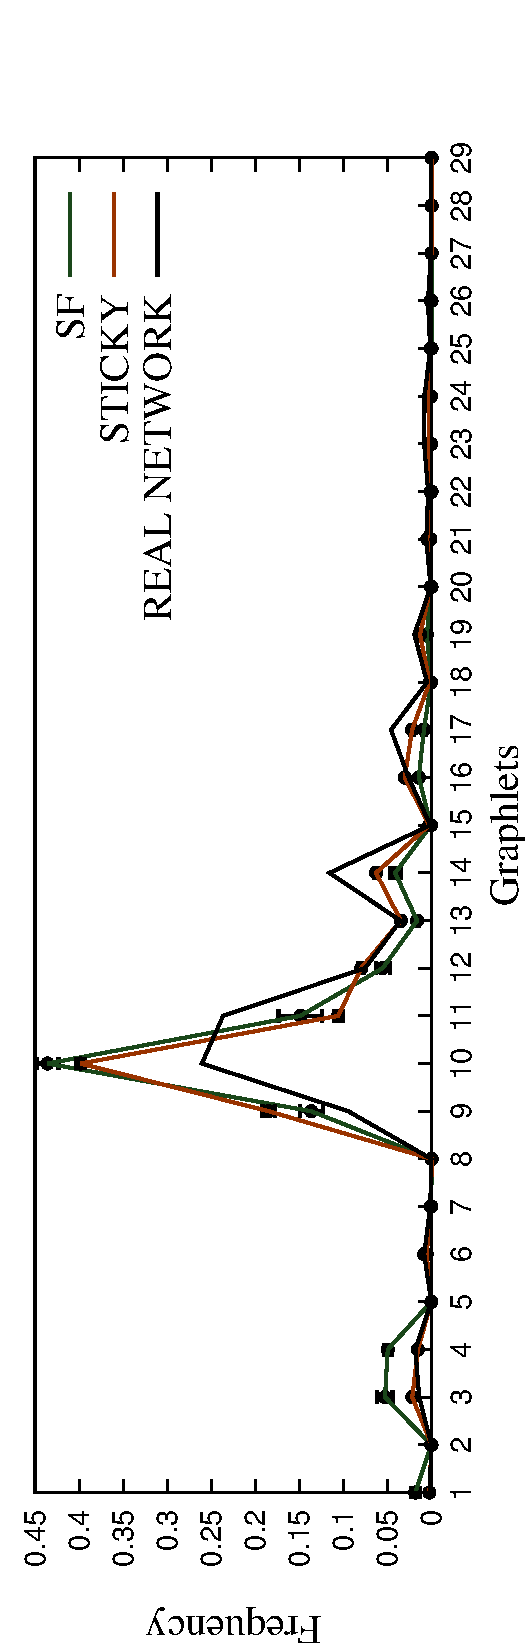
\includegraphics[angle=-90,scale=0.6]{../code/final_results/human_ppi/avg_egdvs_rnd_spreads_figures/spreads_34_rnd2.pdf} 
  \end{subfigure}
\caption[Average GCV for the Human PPI network and ER, ER-DD, GEO, SF and STICKY random models]{Average GCV for the Human PPI network, including the standard deviations displayed as vertical error bars. The random models analysed are: Erd\H{o}s-R\'{e}nyi (ER), Erd\H{o}s-R\'{e}nyi with preserved degree distribution (ER-DD), Geometric (GEO), Scale-free Barab\'{a}si-Albert -- Preferential Attachment (SF) and 
Stickiness-based (STICKY). The length of one vertical bar is equal to one standard deviation $\sigma$. We assume that the samples are normally distributed with mean $\mu$ and variance $\sigma^2$}
\label{ppi_spreads}
\end{figure}

Figure \ref{meta_spreads} shows the average GCVs for the Metabolic networks and the corresponding random networks. We notice that the metabolic networks have a slightly different signature compared to the PPI networks. First of all, they have more graphlets $G_{11}$ but less graphlets $G_{10}$. Secondly, for this class of networks the ER-DD random network seems to be a better approximation according to the GCV signatures, especially for graphlet types \{10,11,12\}. The fact that ER-DD is the best approximation for the Metabolic network is again confirmed in section \ref{rcfd_res}.

\begin{figure}[H]
  \centering
  \textbf{Average GCV for random models of the Human Metabolic network}
  \begin{subfigure}[b]{1.0\textwidth}
    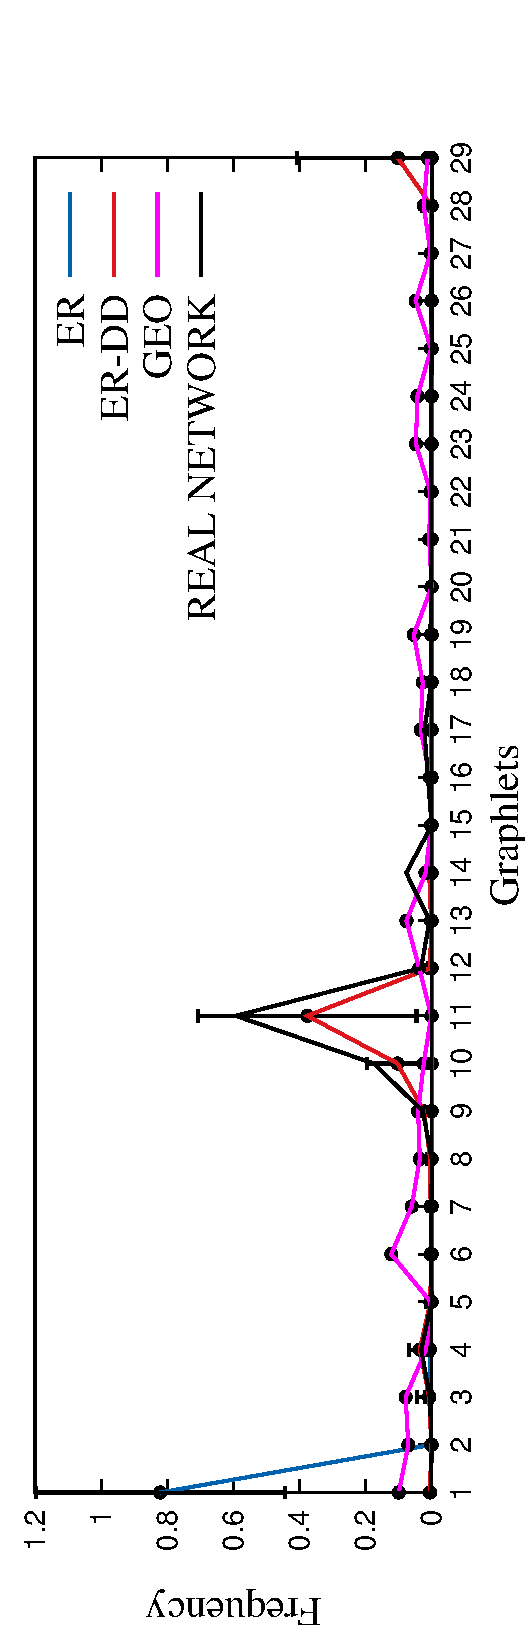
\includegraphics[angle=-90,scale=0.6]{../code/final_results/hsa_metabolic_network/avg_egdvs_rnd_spreads_figures/spreads_012_rnd2.pdf} 
  \end{subfigure}
  \begin{subfigure}[b]{1.0\textwidth}
    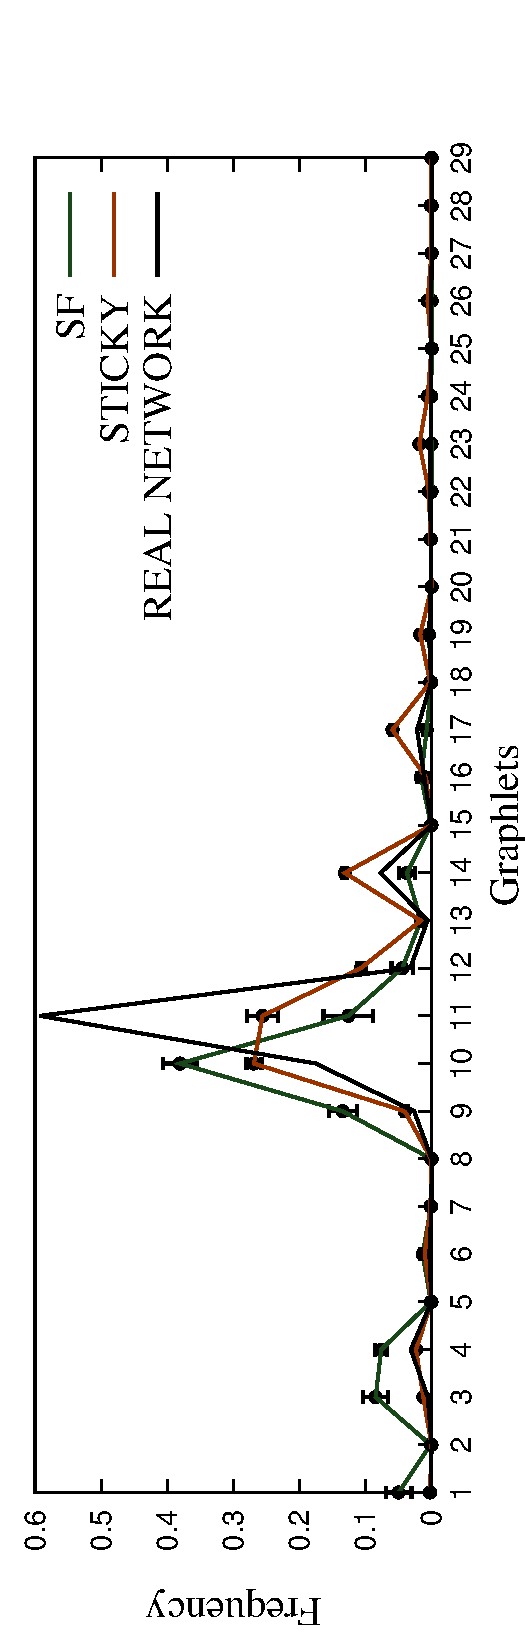
\includegraphics[angle=-90,scale=0.6]{../code/final_results/hsa_metabolic_network/avg_egdvs_rnd_spreads_figures/spreads_34_rnd2.pdf} 
  \end{subfigure}
  \caption[Average GCV for the Human Metabolic network and ER, ER-DD, GEO, SF and STICKY random models]{Average GCV for the Human Metabolic network, including the standard deviations displayed as vertical error bars. The random models analysed are: Erd\H{o}s-R\'{e}nyi (ER), Erd\H{o}s-R\'{e}nyi with preserved degree distribution (ER-DD), Geometric (GEO), Scale-free Barab\'{a}si-Albert -- Preferential Attachment (SF) and Stickiness-based (STICKY). The length of one vertical bar is equal to one standard deviation $\sigma$. We assume that the samples are normally distributed with mean $\mu$ and variance $\sigma^2$}
  \label{meta_spreads}
\end{figure}

Figure \ref{trade_spreads} shows the average GCVs for the WTNs and the corresponding random graphs. Surprisingly, for this type of networks we see a greater variety in the frequencies of graphlets, with graphlets in the 15--29 range now being much more represented than in the biological networks. The simple Erd\H{o}s-R\'{e}nyi model has a large variance for the frequency of graphlets \{3,9,10\}. On the other hand, the Erd\H{o}s-R\'{e}nyi graphs with preserved degree distribution offer a good GCV signature approximation, especially for graphlets in the range \{9-18\}, which are the 5-node graphlets at the sparse end of the spectrum. The Stickiness-based random graphs also offer a good approximation, a result that is confirmed by the \emph{Relative Cluster Frequency Agreement} in section \ref{rcfd_res}.

\begin{figure}[H]
  \centering
  \textbf{Average GCV for random models of the 2010 World Trade Networks}
  \begin{subfigure}[b]{1.0\textwidth}
    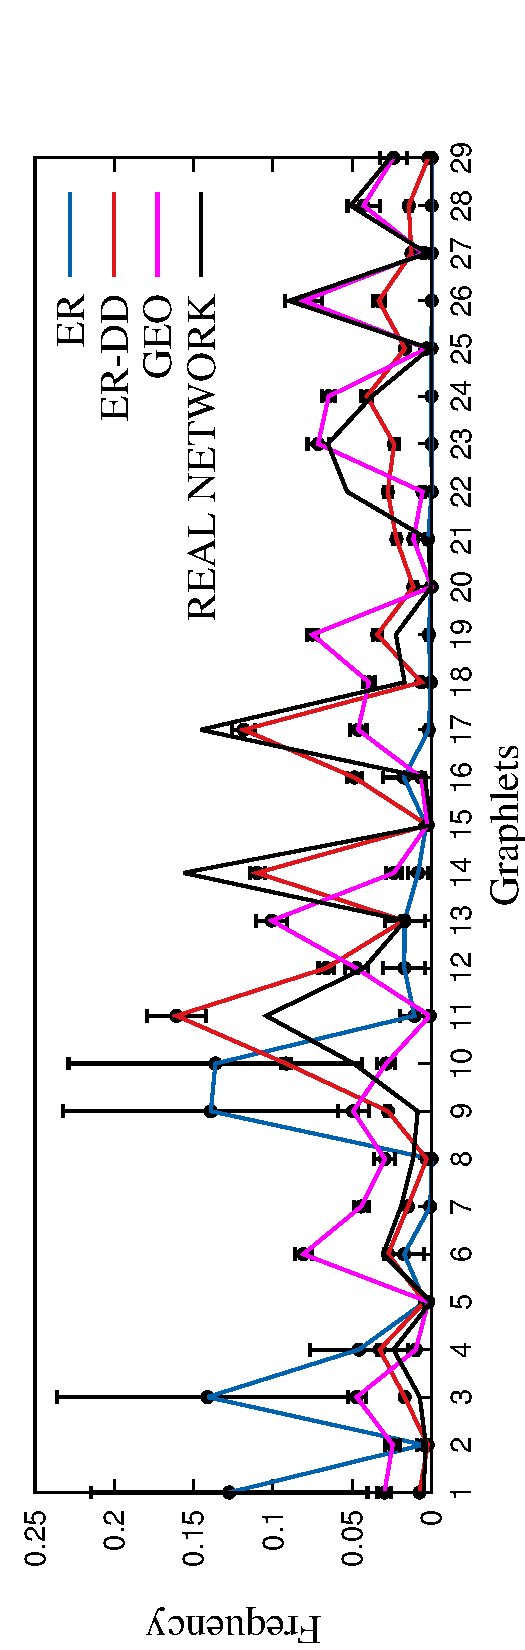
\includegraphics[angle=-90,scale=0.6]{../code/final_results/trade_2010_thresholded/avg_egdvs_rnd_spreads_figures/spreads_012_rnd2.pdf} 
  \end{subfigure}
  \begin{subfigure}[b]{1.0\textwidth}
    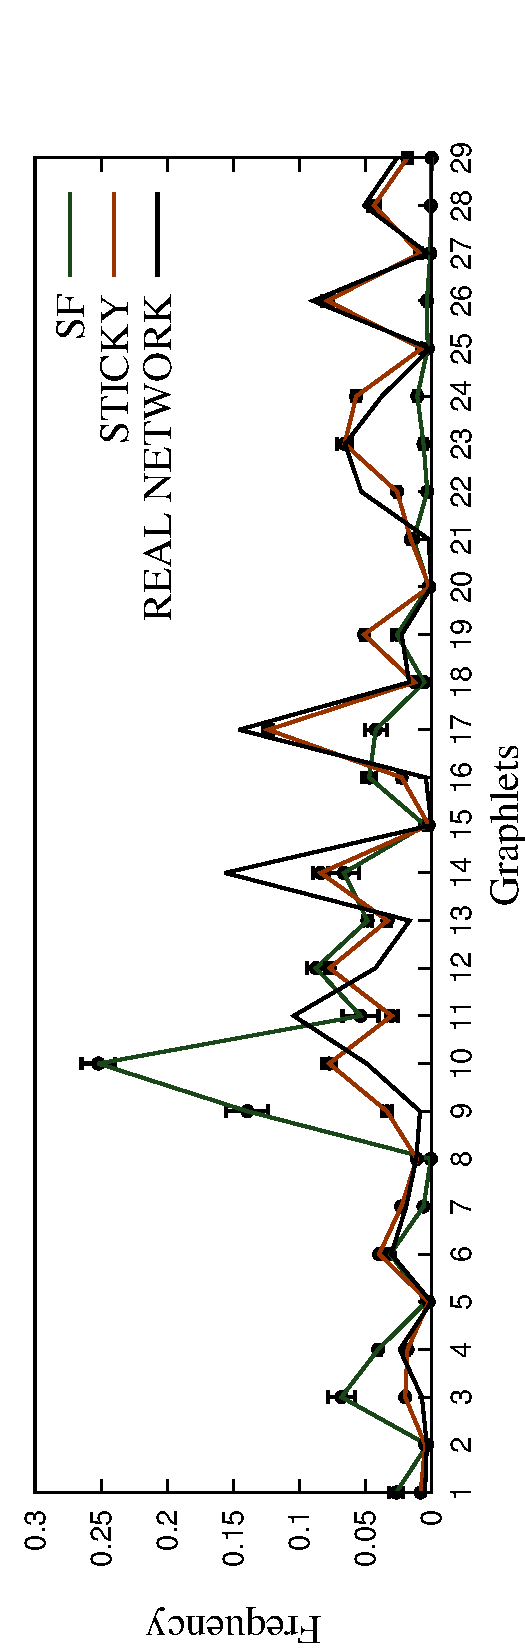
\includegraphics[angle=-90,scale=0.6]{../code/final_results/trade_2010_thresholded/avg_egdvs_rnd_spreads_figures/spreads_34_rnd2.pdf} 
  \end{subfigure}
  \caption[Average GCV for the World Trade network and ER, ER-DD, GEO, SF and STICKY random models]{Average GCV for the 2010 WTN, including the standard deviations displayed as vertical error bars. The random models analysed are: Erd\H{o}s-R\'{e}nyi (ER), Erd\H{o}s-R\'{e}nyi with preserved degree distribution (ER-DD), Geometric (GEO), Scale-free Barab\'{a}si-Albert -- Preferential Attachment (SF) and 
Stickiness-based (STICKY). The length of one vertical bar is equal to one standard deviation $\sigma$. We assume that the samples are normally distributed with mean $\mu$ and variance $\sigma^2$}
  \label{trade_spreads}
\end{figure}


\subsection{Relative Cluster Frequency Distance Results}
\label{rcfd_res}

The \emph{Relative Cluster Frequency Distance} (RCFD) between two GCV vectors is a measure of how different they are with each other. It it is defined as the Euclidean norm of the difference between the two GCV vectors. A low RCFD value means that the signatures are similar to each other, while a high value means that the signatures are different. See section \ref{rcfd} for the exact definition of RCFD. When applied to the average GCV signature of two networks, RCFD can tell us how similar or different the two networks are. The question we are trying to answer here is: according to the average GCV signature, which random graph is best for modelling the real underlying network? The three tables from figure \ref{gcv_agr} show the RCFD distances between the real network and random models\footnote{the real network has been used to generate these random models}, applied to our three main classes of networks: PPI, Metabolic and World Trade. 

For the Human PPI network (table (\subref{tab:rcfd_ppi}) from fig \ref{gcv_agr}), the random networks that best approximate the real network are the Stickiness-based (STICKY) random networks, having the smallest RCFD of 0.492, while the Scale-free Barab\'{a}si-Albert (SF) graphs also offer a good approximation of the original network, having a RCFD of 0.607. The other random models perform much worse in this respect because they cannot capture all the underlying complexity in the dataset. Moreover, we also notice that the difference between the SF and STICKY GCV signatures is really small (0.329), meaning that the generated networks are topologically similar to each other.

For the Human Metabolic network (table (\subref{tab:rcfd_meta}) from fig \ref{gcv_agr}), the results are slightly different. The best-performing random networks are the ER-DD (RCFD to the real network is 0.557), built using the "stubs" method (see section \ref{er-dd}). The second-best random network is the STICKY model which has an RCFD between itself and the Real network of 0.697. When analysing the 2010 WTN between countries(table (\subref{tab:rcfd_trade}) from fig \ref{gcv_agr}), the random network with the best approximation to the real network is again the Stickiness-based network, followed closely by Erd\H{o}s-R\'{e}nyi with preserved degree distribution.

We therefore conclude that the STICKY random model is best at modelling PPI and WTN networks, while ER-DD is best at modelling Metabolic networks.

\rowcolors{1}{blue1}{blue2}

%     Relative Cluster Frequency Distance for the Human PPI network\\
\newcommand{\humanppiagr}{% Just for this example
      \begin{tabular}{ c | c  c  c  c  c | c }
      Model & ER & ER DD & GEO & SF & STICKY & REAL\\
      \hline
      ER     & 0.000 & 1.296 & 1.889 & 1.963 & 1.995 & 1.995 \\
      ER DD  & 1.296 & 0.000 & 1.554 & 1.018 & 1.233 & 1.191 \\
      GEO    & 1.889 & 1.554 & 0.000 & 1.413 & 1.406 & 1.311 \\
      SF     & 1.963 & 1.018 & 1.413 & 0.000 & 0.329 & 0.607 \\
      STICKY & 1.995 & 1.233 & 1.406 & 0.329 & 0.000 & \textbf{0.492} \\
      \hline
      REAL   & 1.995 & 1.191 & 1.311 & 0.607 & \textbf{0.492} & 0.000\\
      \end{tabular}
}

%     Relative Cluster Frequency Distance for the Human Metabolic network\\
\newcommand{\hsametaagr}{% Just for this example
    \begin{tabular}{ c | c  c  c  c  c | c }
    Model & ER & ER DD & GEO & SF & STICKY & REAL\\
    \hline
    ER     & 0.000 & 1.499 & 1.610 & 1.709 & 1.804 & 1.807\\
    ER DD  & 1.499 & 0.000 & 1.430 & 1.040 & 0.799 & \textbf{0.557}\\ 
    GEO    & 1.610 & 1.430 & 0.000 & 1.356 & 1.438 & 1.648\\
    SF     & 1.709 & 1.040 & 1.356 & 0.000 & 0.784 & 1.054\\
    STICKY & 1.804 & 0.799 & 1.438 & 0.784 & 0.000 & 0.697\\
    \hline
    REAL   & 1.807 & \textbf{0.557} & 1.648 & 1.054 & 0.697 & 0.000\\
    \end{tabular}
}

%     Relative Cluster Frequency Distance for the Trade 2010 thresholded network\\
\newcommand{\tradeagr}{% Just for this example
    \begin{tabular}{ c | c  c  c  c  c | c }
    Model & ER & ER DD & GEO & SF & STICKY & REAL\\
    \hline
    ER     & 0.000 & 1.134 & 1.198 & 0.663 & 1.172 & 1.336 \\
    ER DD  & 1.134 & 0.000 & 1.065 & 0.819 & 0.490 & 0.572 \\
    GEO    & 1.198 & 1.065 & 0.000 & 1.099 & 0.609 & 0.873 \\
    SF     & 0.663 & 0.819 & 1.099 & 0.000 & 0.896 & 1.161 \\
    STICKY & 1.172 & 0.490 & 0.609 & 0.896 & 0.000 & \textbf{0.465} \\
    \hline
    REAL   & 1.336 & 0.572 & 0.873 & 1.161 & \textbf{0.465} & 0.000\\
    \end{tabular}

}


\begin{figure}[H]%
  \centering
  \vspace{1em}
  \begin{subfigure}{1.0\textwidth}
    \centering
    \humanppiagr   
    \caption{RCFD distances for the Human PPI network}
    \vspace{1.5em}
    \label{tab:rcfd_ppi}
  \end{subfigure}
%   \qquad
%   \hspace{5em}
  \begin{subfigure}{1.0\textwidth}
    \centering
    \hsametaagr   
    \caption{RCFD distances for the Human Metabolic network}
    \vspace{1.5em}
    \label{tab:rcfd_meta}
  \end{subfigure}
%   \vspace{1em}
  \begin{subfigure}{1.0\textwidth}
    \centering
    \tradeagr 
    \caption{RCFD distances for the 2010 World Trade network}
    \label{tab:rcfd_trade}
  \end{subfigure}
%   \subfloat[][]{}
%   \qquad
%   \subfloat[][]{}
  \caption[RCFD distances for the Human PPI, Human Metabolic and WTN networks.]{The RCFD distances for (\subref{tab:rcfd_ppi}) Human PPI network (\subref{tab:rcfd_meta}) Human Metabolic network (\subref{tab:rcfd_trade}) 2010 WTN and five model networks: Erd\H{o}s-R\'{e}nyi (ER), Erd\H{o}s-R\'{e}nyi with preserved degree distribution (ER DD), Geometric (GEO), Scale-Free - Barab\'{a}si-Albert Preferential Attachment (SF) and Stickiness-based (STICKY). For each network class, we have calculated not only the distance between every pair of random network models, but also the distance between every random network model and the real network which was used to generate the random models.}
  \label{gcv_agr}%
\end{figure}

% \begin{figure}[H]%
%   \centering
%   \subfloat[][]{\humanppiagr}
%   \qquad
%   \subfloat[][]{\hsametaagr}
%   \qquad
%   \subfloat[][]{\tradeagr}
%   \caption[RCFD distances for the Human PPI, Human Metabolic and WTN networks.]{The RCFD distances for (a) Human PPI network (b) Human Metabolic network (c) 2010 WTN and five model networks: Erd\H{o}s-R\'{e}nyi (ER), Erd\H{o}s-R\'{e}nyi with preserved degree distribution (ER DD), Geometric (GEO), Scale-Free - Barab\'{a}si-Albert Preferential Attachment (SF) and Stickiness-based (STICKY). For each network class, we have calculated not only the distance between every pair of random network models, but also between every random network model and the real network which was used to generate the random models}
%   \label{gcv_agr}%
% \end{figure}



\section{World Trade networks}
\label{trade_res_heatmaps}

After running initial experiments that study the average GCV of a network, we performed experiments that were specific to each of the network classes. In this section, we present the main results obtained for the World Trade Networks (WTNs). A brief summary of these networks is given in section \ref{sec:trade_bck}. 

\begin{figure}[H]
  \begin{center}
  \hbox{\hspace{-1cm}
  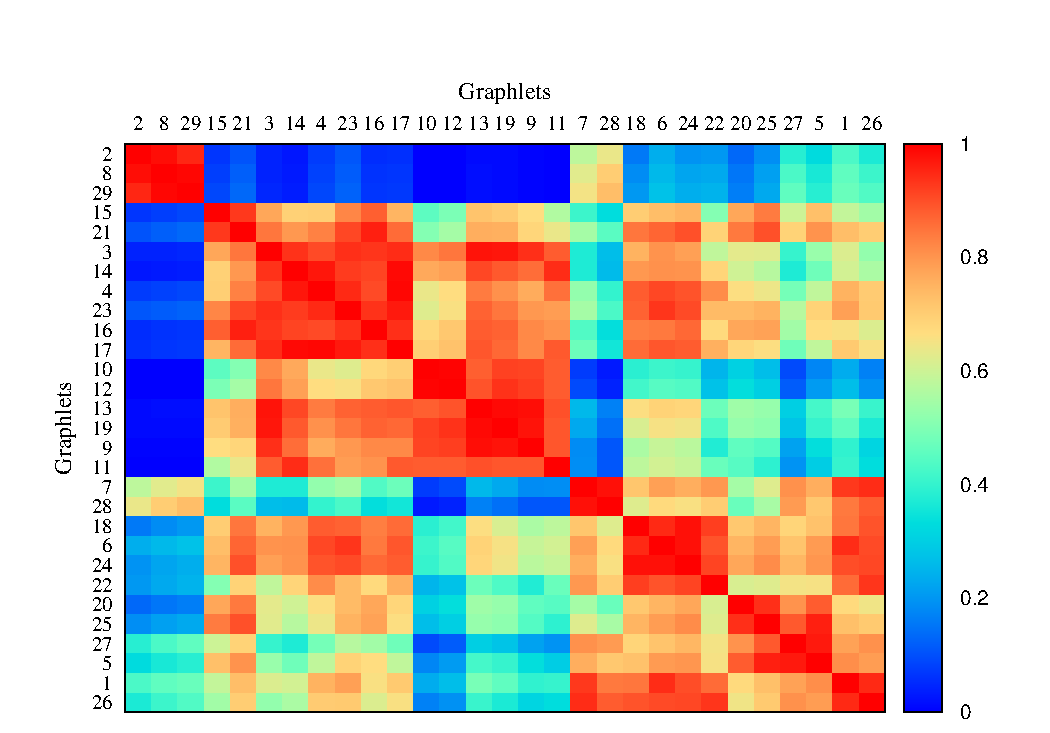
\includegraphics[scale=1.0]{../code/final_results/trade_2010_thresholded/heatmap_pearsons_hclust_trade_2010_thresholded-poly-32.pdf}} 
  \caption[Pearson's GCV correlation matrix for the 2010 WTN]{Pearson's GCV correlation matrix for the 2010 WTN. It has been normalised with feature scaling and a $3^{rd}$ degree polynomial, and then hierarchically clustered with complete linkage.}
  \label{fig:trade_heatmap}
  \end{center}
\end{figure}


Figure \ref{fig:trade_heatmap} shows the \emph{Pearson's GCV Correlation matrix} for the 2010 WTN. This correlation matrix was normalised with feature scaling and a $3^{rd}$ degree polynomial function. For details on how this has been calculated see the methodology section \ref{sec:metho_pears}. Other polynomial functions have been tested, but the $3^{rd}$ degree polynomial was the most effective in emphasising the clusters of graphlets that are formed on the diagonal. These clusters of graphlets are as follows:
\begin{itemize}
 \item Cliques cluster made of graphlets \{2,8,29\}.
 \item A cluster that is made of graphlets \{15,21,3,14,4,23,16,17,10,12,13,19,9,11\} which can be split into 2 further sub-clusters: 
    \begin{itemize}
     \item $P_4$ cluster made of graphlets \{15,21,3,14,4,23,16,17\}. These are all 
     graphlets that contain a $P_4$ (path of 4 nodes, graphlet $G_3$). 
     \item Claw\footnote{A claw $C_n$ is a graphlet that has a central node and $n-1$ satellite nodes connected to it. See section \ref{graph_terminology} for a full definition.} cluster made of \{10,12,13,19,9,11\}. These graphlets all contain a $C_3$ ( claw on 3 nodes, graphlet $G_4$)
    \end{itemize}
 \item A cluster that is made of graphlets \{20,25,27,5\}. These graphlets all contain an $S_4$ (cycle of 4 nodes).   
 \item Another set of graphlets that correlate is \{18,6,24,22,1,26\}. The reason why graphlets \{1,26\} have been added is because they also correlate with the other cluster, even if they are not right next to them in the heat map. These all contain at least one $P_3$ (path of 3 nodes).
\end{itemize}

Now that we know which graphlets cluster together, we will use these results in the subsequent CCA analysis in section \ref{sec:cca_orig}.

\subsection{Correlation matrix change during 1962--2010}
\label{trade_change_orig}

%gcv offset: -2   Spearman's rank coefficient: corr: -0.493973099551    p_value: 0.000485081849961
The results from the previous section were concerned with the correlation matrix of the 2010 WTN. However, we are also interested to see how graphlets correlate in WTNs from other years. We therefore compute the Pearson's GCV correlation matrix for all the yearly WTNs in the period 1962--2010. Using the 49 different correlation matrices, we then compute the \emph{change in the correlation matrix} during the respective time frame. In order to calculate the change in correlation matrix between year $Y$ and $Y+1$, we simply subtract in a pairwise manner the two matrices and then return the sum of squares of all the elements in the matrix. For the exact formula used see equation \ref{pears_matrix_diff} from section \ref{pearsons_background}. 

We then tried to find out if there is any correlation between the network topology and Crude Oil price. If one of these attributes changes, it might be possible that the other reacts. However, this might happen with a certain number of years delay. In order to account for this, we shift the vector of GCV correlation change by [-2,-1,0,1,2] years. For each of these 5 cases, we calculate the \emph{Spearman's rank correlation coefficient} and the respective p-value for the following vectors:
\begin{itemize}
 \item one 48-element vector containing the \emph{change in Pearson's GCV correlation matrix}
 \item one 48-element vector containing the \emph{change in the price of Crude Oil}
\end{itemize}


The best correlation is obtained when the vector of GCV correlation is shifted by -2 years. This scenario is plotted in figure \ref{change_over_time_orig}. Surprisingly, the oil change in inversely correlated with the change in network topology: the Spearman's rank correlation coefficient is -0.49, having a p-value of 0.0004. Since the p-value is smaller than 0.05, the result is statistically significant. The explanation for this is as follows: high oil prices generally have a large negative impact on the global economic growth. Slower growth leads to diminished investment-related activity in the countries affected, which in turn deters the creation of new trading partners. This implies that the network structure remains mostly unchanged, a fact that results in a low GCV correlation change. Moreover, because the best correlation is obtained when the change in GCV is shifted by -2 years, this might suggest that changes in network structure cause the Crude Oil price to change. However, we did not have time to 
perform more supporting experiments in order to validate the causality aspect of this claim.

Furthermore, there are several major economic events for which we do not have a big change in the topology of our network, such as the 2007 sub-prime mortgage crisis or the 1997 Asian financial crisis. This implies that the unnormalised Pearson's GCV correlation matrix is not affected by these major events. Similar results that use a normalised version of the GCV are better correlated with global economic and social events (see section \ref{rev_trade_change}).

\begin{figure}[H]
  \centering
  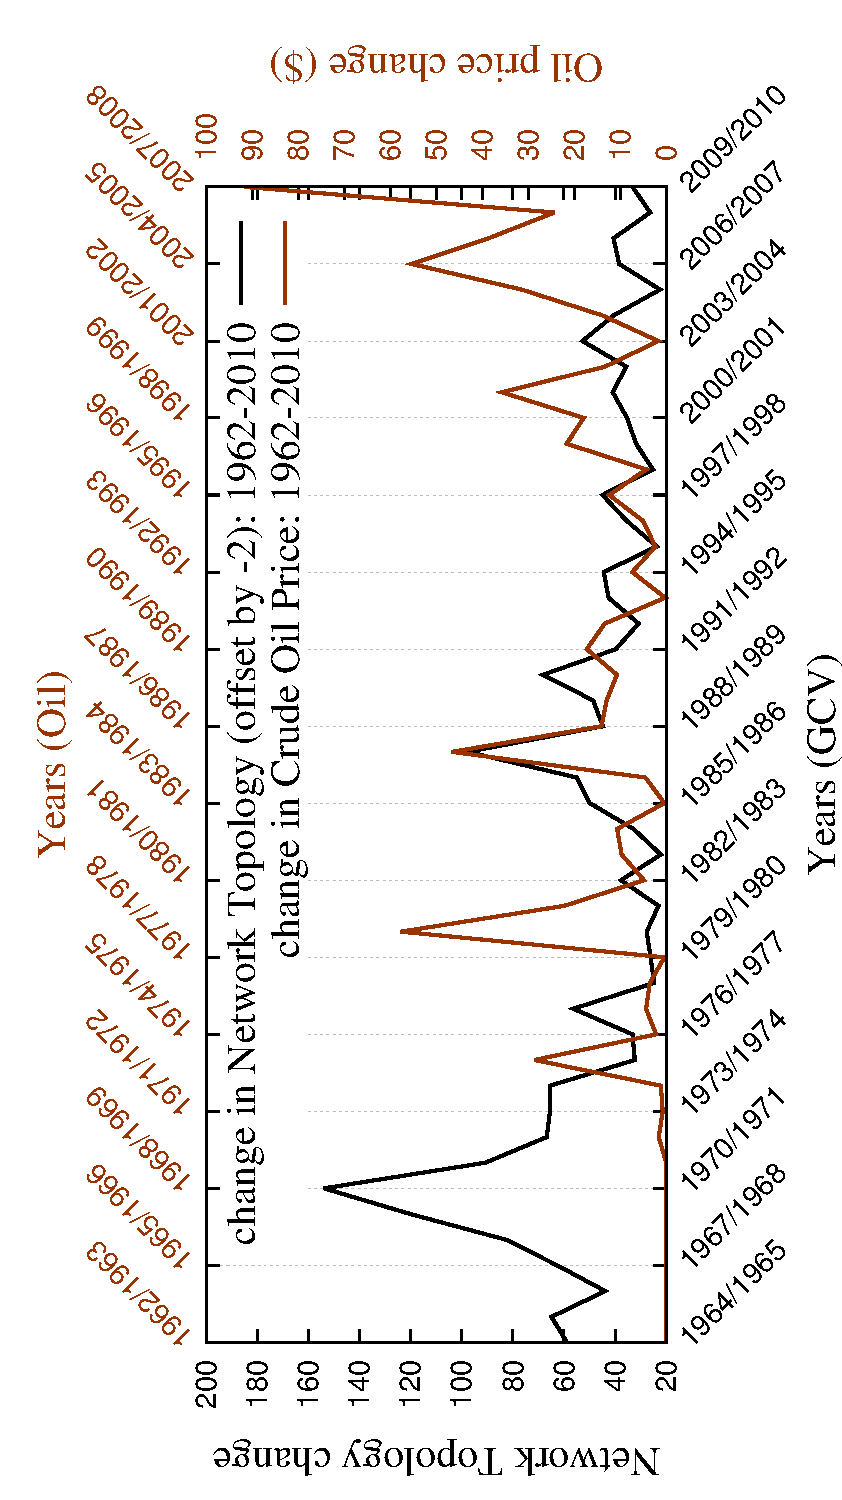
\includegraphics[angle=-90,scale=0.6]{../code/final_results/all_trade_thresh/change_over_time2}
% \mbox{\epsfbox{../code/final_results/all_trade_thresh/change_over_time}}
\caption[Evolution of WTN structure during 1962--2010 - unnormalised GCV]{Evolution of WTN structure during 1962--2010 using the unnormalised GCV. Plotted in black is the change in GCV correlation that has been offset by -2 years, while the change in Crude Oil Price is plotted in brown. Spearman's rank coefficient between oil price change and change in network topology is -0.49 with a p-value of 0.0004. This suggests that when the change in GCV correlation between countries changes, then the oil price stays the same. The top and left axis tics correspond to the Oil curve, while the bottom and the left axis tics correspond to the network topology curve.}
\label{change_over_time_orig}
\end{figure}

% Omer - 1993 is computed as (Price_{1993} - Price_{1992}). The graph however shows 1993/1992 or smth similar

\subsection{CCA - 1980--2010 World Trade networks}
\label{sec:cca_orig}
After correlating graphlets from the GCV vector with each other in order to see which one of them have a similar behaviour, the next step is to correlate the GCV vectors with the economic indicators of a country. This can be done using \emph{Canonical Correlation Analysis} (CCA) which is described in section \ref{cca_background}. The two variates we correlated are:
\begin{enumerate}
 \item the X variate containing economic indicators (GDP per Capita, Level of Employment). See section \ref{sec:trade_bck} for details about all the economic indicators used.
 \item the Y variate containing the unnormalised GCV vectors for each country.
\end{enumerate}

The CCA analysis uses data for 119 countries over a period of 30 years (1980-2010). Each country-year pair represents one sample for which we have both economic indicators (X variate) and the GCV (Y variate).



\newcommand{\ccaIndicatorsTradeUnnorm}{
  \begin{tabular}{r}
  \cellcolor{black}\textcolor{ccacol1}{POP}\\
  \cellcolor{black}\textcolor{ccacol1}{LE}\\
  \cellcolor{black}\textcolor{ccacol1}{KI x RGDPL x POP}\\
  \cellcolor{black}\textcolor{ccacol1}{RGDPCH x POP}\\
  \cellcolor{black}\textcolor{ccacol1}{RGDPL x POP}\\
  \cellcolor{black}\textcolor{ccacol1}{RGDPL2 x POP}\\
  \cellcolor{black}\textcolor{ccacol1}{KC x RGDPL x POP}\\
  \cellcolor{black}\textcolor{ccacol1}{KG x RGDPL x POP}\\
  \cellcolor{black}\textcolor{ccacol2}{KC x RGDPL}\\
  \cellcolor{black}\textcolor{ccacol3}{RGDPCH}\\
  \cellcolor{black}\textcolor{ccacol3}{RGDPL}\\
  \cellcolor{black}\textcolor{ccacol3}{RGDPL2}\\
  \cellcolor{black}\textcolor{ccacol3}{KG x RGDPL}\\
  \cellcolor{black}\textcolor{ccacol4}{KI x RGDPL}\\
  \cellcolor{black}\textcolor{ccacol4}{XRAT}\\
  \cellcolor{black}\textcolor{ccacol4}{KC}\\
  \cellcolor{black}\textcolor{ccacol5}{KI}\\
  \cellcolor{black}\textcolor{ccacol5}{BCA per RGDPL}\\
  \cellcolor{black}\textcolor{ccacol5}{KG}\\
  \cellcolor{black}\textcolor{ccacol6}{BCA}\\
  \cellcolor{black}\textcolor{ccacol6}{OPENK}
  \end{tabular}

}


\begin{figure}[H]
  \centering
    \begin{tikzpicture}[scale=\ccafigscale,show background rectangle, 
  background rectangle/.style={fill=black},
  color=white,help lines/.style={color=lightgray,line width=0.2pt},post/.style={->,shorten >=1pt,>=stealth',thick}]

    \node[upper left,inner sep=0,scale=\ccafigscale] (indicators) at (-2.0,0) {\ccaIndicatorsTradeUnnorm};	
    \shade[top color=green,bottom color=yellow] (4,0) rectangle (4.5,5);
    \shade[top color=yellow,bottom color=red] (4,-5) rectangle (4.5,0);
    \node[upper left,inner sep=0] (dummy) at (13.0,4) {}; % for extending the black bounding box
    \node[upper left,inner sep=0,scale=\ccafigscale * 1.3] (corr_text) at (4.25,-6.0) {Correlation};
    \node[upper left,inner sep=0,red] (corr_text) at (4.25,-5.5) {-1};
    \node[upper left,inner sep=0, green] (corr_text) at (4.25,5.5) {1};
    \node[upper left,inner sep=0] (corr_text) at (4.75,0) {0};
    
    \node[upper left,inner sep=0,scale=\ccafigscale] (g1) at (7.5,5) {\gonecca{ccacol1}};
    \node[upper left,inner sep=0,scale=\ccafigscale] (g2) at (10.5,3.5) {\gtwocca{ccacol1}};
    \node[upper left,inner sep=0,scale=\ccafigscale] (g6) at (7.5,2) {\gsixcca{ccacol1}};
    \node[upper left,inner sep=0,scale=\ccafigscale] (g16) at (10.5,-2.5) {\gsixteencca{ccacol3}};
    \node[upper left,inner sep=0,scale=\ccafigscale] (g15) at (7.5,-4) {\gfifteencca{ccacol3}};
    \node[upper left,inner sep=0,scale=\ccafigscale] (g20) at (10.5,-5.5) {\gtwentycca{ccacol3}};
    
    \draw[line,color=white] (6,0) -- (13.00,0);
    \node[upper left,inner sep=0,scale=\ccafigscale * 1.3] (strong_corr) at (10,0.5) {Highest correlations};    
    \node[upper left,inner sep=0,scale=\ccafigscale * 1.3] (strong_corr) at (10,-0.5) {Lowest correlations};    
    
    \draw[line,color=ccacol1] (0.00,4.80) -| (1.64,3.83) -- (4.00,3.83);
    \draw[line,color=ccacol1] (0.00,4.33) -| (1.15,3.79) -- (4.00,3.79);
    \draw[line,color=ccacol1] (0.00,3.85) -| (0.8,3.63) -- (4.00,3.63);
    \draw[line,color=ccacol1] (0.00,3.38) -| (0.8,3.59) -- (4.00,3.59);
    \draw[line,color=ccacol1] (0.00,2.90) -| (1.2,3.59) -- (4.00,3.59);
    \draw[line,color=ccacol1] (0.00,2.42) -| (1.3,3.58) -- (4.00,3.58);
    \draw[line,color=ccacol1] (0.00,1.95) -| (1.4,3.50) -- (4.00,3.50);
    \draw[line,color=ccacol1] (0.00,1.48) -| (1.5,3.47) -- (4.00,3.47);
    \draw[line,color=ccacol2] (0.00,1.00) -| (1.6,2.10) -- (4.00,2.10);
    \draw[line,color=ccacol3] (0.00,0.53) -| (1.7,1.33) -- (4.00,1.33);
    \draw[line,color=ccacol3] (0.00,0.05) -| (1.9,1.33) -- (4.00,1.33);
    \draw[line,color=ccacol3] (0.00,-0.42) -| (2.1,1.33) -- (4.00,1.33);
    \draw[line,color=ccacol3] (0.00,-0.90) -| (2.3,1.09) -- (4.00,1.09);
    \draw[line,color=ccacol4] (0.00,-1.38) -| (2.5,0.89) -- (4.00,0.89);
    \draw[line,color=ccacol4] (0.00,-1.85) -| (2.7,0.60) -- (4.00,0.60);
    \draw[line,color=ccacol4] (0.00,-2.33) -| (2.8,0.49) -- (4.00,0.49);
    \draw[line,color=ccacol5] (0.00,-2.80) -| (3,-0.30) -- (4.00,-0.30);
    \draw[line,color=ccacol5] (0.00,-3.27) -| (3.2,-0.74) -- (4.00,-0.74);
    \draw[line,color=ccacol5] (0.00,-3.75) -| (3.4,-0.87) -- (4.00,-0.87);
    \draw[line,color=ccacol6] (0.00,-4.23) -| (3.6,-1.00) -- (4.00,-1.00);
    \draw[line,color=ccacol6] (0.00,-4.70) -| (3.8,-1.24) -- (4.00,-1.24);



    
    
    \draw[line,color=ccacol1] (g1) -| (6.1,4.2) -- (4.5,4.2);
    \draw[line,color=ccacol1] (g2) -| (5.9,4.05) -- (4.5,4.05);
    \draw[line,color=ccacol1] (g6) -| (5.7,4.0) -- (4.5,4.0);

    \draw[line,color=ccacol3] (g16) -| (5.5,2.8) -- (4.5,2.8);
    \draw[line,color=ccacol3] (g15) -| (5.3,2.5) -- (4.5,2.5);
    \draw[line,color=ccacol3] (g20) -| (5.1,2.2) -- (4.5,2.2);
    
    \end{tikzpicture}
    \caption[CCA - World Trade networks - unnormalised GCV - Picture version]{Canonical Correlation Analysis between economic indicators and the GCV signature. Only the graphlets that have the highest respectively lowest cross-loadings are shown in the picture. However, all the graphlets have positive cross-loadings, with the lowest cross-loading having a value of 0.44. Openness (OPENK), Balance Current Account (BCA) and a few other indicators correlate negatively with all the graphlets, because their cross-loadings have different signs. On the other hand, the rest of the indicators such as Population (POP), Level of Employment (LE) and GDP per capita (RGPDL, RGDPCH) correlate positively with all the graphlets, since their cross-loadings have the same sign. The overall correlation is 0.89 with a p-value smaller than 0.0001. This result suggests that big and wealthy countries have a large network of trading partners that is rich in graphlets.}
    \label{fig:all_trade_cca_unnorm_black}	
\end{figure}


CCA results are presented in figure \ref{fig:all_trade_cca_unnorm_black}. A supplementary table with the list of all the cross-loadings can be found in figure \ref{all_trade_thresh_cca_orig} in the appendix. This result shows that all the graphlets correlate positively\footnote{An element from the $X$ variate correlates positively with another element from the $Y$ variate if and only if their cross-loadings have the same sign} with some indicators such as Population, Level of Employment or GDP per capita and negatively with Trade Openness and Balance of Current Account. This means that big and rich countries that have a high population and GDP per capita have a neighbourhood rich in graphlets, while small and poor countries with account deficits have a neighbourhood sparse in graphlets. The population of the country seems to be quite an important factor for determining whether it will have a rich neighbourhood because of the following two reasons:
\begin{itemize}
 \item In the $X$ variate, population has the weight with the highest magnitude: 0.766
 \item Most of the other economic indicators that have a high weight are obtained by multiplying population with other indicators. This is also the case in a similar CCA Analysis of Yavero\u{g}lu et al. using graphlet orbits \cite{yaverouglu2014revealing}.
\end{itemize}

\subsection{Economic Integration}
\label{sec:cca_integration}

We now try to find out if the level of \emph{Economic Integration} of a country is positively correlated with dense graphlets and negatively correlated with sparse graphlets. This is something to be expected, because when a country is part of a strong trading bloc, it's neighbours have a higher probability of doing heavy trade with one another. This is because there is incentive for the country to trade more with the partners from the same bloc, that are already trading a lot with each other. This would in turn result in denser graphlets in the neighbourhood of that country. The idea of correlating the GCV with the integration level of a country was entirely mine.

For a given country, there exist several stages of economic integration. One possible classification is the following:
\begin{enumerate}
 \item no economic integration 
 \item Multilateral Free Trade Area (e.g. AFTA, CEFTA, CISFTA)
 \item Customs union (e.g. EAC, EUCU, MERCOSUR)
 \item Common market (e.g. EEA, EFTA) 
 \item Customs and Monetary Union (e.g. CEMAC/franc, UEMOA/franc) 
 \item Economic union (e.g. CSME, EU) 
 \item Economic and monetary union (e.g. CSME + EC dollar, EU + euro)
\end{enumerate}

We found some preliminary data on the Internet which labels each country using the most advanced integration agreement it signed. Using this data, we computed an integration index (1-7) for each country and correlated it with the GCV signature using CCA.


\begin{figure}
  \begin{subfigure}{.65\textwidth}
  \centering
  \begin{tabular}{ c c | c c }
    \multicolumn{2}{c}{Canonical Correlation} &  \multicolumn{2}{c}{0.61882} \\
    \multicolumn{2}{c}{p-value} &  \multicolumn{2}{c}{0.01280} \\
    \hline
    \multicolumn{2}{c}{X variate} & \multicolumn{2}{c}{Y variate}\\
    \hline
  Integration & 0.61882 &  G29 & 0.28704\\
  & &  G8 & 0.28349\\
  & &  G2 & 0.27862\\
  & &  G22 & 0.26820\\
  & &  G28 & 0.26806\\
  & &  G7 & 0.26021\\
  & &  G26 & 0.26011\\
  & &  G18 & 0.24661\\
  & &  G1 & 0.23837\\
  & &  G24 & 0.23133\\
  & &  G6 & 0.22969\\
  & &  G4 & 0.22021\\
  & &  G27 & 0.22013\\
  & &  G17 & 0.21021\\
  & &  G14 & 0.20631\\
  & &  G23 & 0.20420\\
  & &  G5 & 0.20149\\
  & &  G20 & 0.19391\\
  & &  G25 & 0.19122\\
  & &  G21 & 0.19076\\
  & &  G16 & 0.19026\\
  & &  G11 & 0.18330\\
  & &  G3 & 0.17730\\
  & &  G15 & 0.16814\\
  & &  G13 & 0.16764\\
  & &  G19 & 0.16051\\
  & &  G9 & 0.15087\\
  & &  G12 & 0.14886\\
  & &  G10 & 0.14638\\
  \end{tabular}

  \end{subfigure}
  \begin{subfigure}{.25\textwidth}
    \centering 
    \rowcolors{1}{}{}		
    
    \gtwentynine
    \geight
    \gtwo
    \gdots
    \gnine
    \gtwelve
    \gten

  \end{subfigure}
  
\caption[CCA - World Trade Network - Integration index]{CCA results between the Integration index ($X$ variate) and the GCV ($Y$ variate). The Integration index of a country is positively correlated with all the graphlets. However, the strongest correlation is with dense graphlets such as cliques \{29,8,2\} because they have the highest weight, while sparser graphlets \{10,12,9\} have the lowest weight. The overall correlation is 0.61, with a p-value of 0.01, suggesting the correlation is statistically significant.}
\label{trade_2010_thresholded_cca}
\end{figure}


Figure \ref{trade_2010_thresholded_cca} presents these preliminary CCA results. They confirmed our initial expectations, with dense graphlets correlating most with the integration index, while the sparse graphlets correlating least. However, since the source of the data that was used for this experiment could not be verified, we searched for an official index that quantifies political integration for each country around the world. Although we haven't found an index that uses the 6-level scale that we previously mentioned, we found some indices on the \emph{World Trade Organisation} website that measure the number of \emph{Regional Trade Agreements} (RTAs) of a country \cite{rtas2014wto}. These RTAs are defined as trade agreements that are concluded between countries that are geographically close to each other\footnote{However, the countries do not strictly have to be geographically close in order to sign an RTA.}. For a given country, the number of RTAs gives us a measure of economic and political 
integration, since these agreements are mainly signed within trading blocks. The RTAs facilitate trade on a regional basis and can be of several types:
\begin{itemize}
 \item A Free Trade Agreement (FTA)
 \item A Customs Union (CU)
 \item Economic Integration Agreement (EIA)
 \item Partial Scope Agreement\footnote{Covers only certain types of products} (PS)
\end{itemize}

The \emph{World Trade Organisation} provides indices for each of the following classes of RTAs:
\begin{itemize}
 \item Goods RTAs: agreements that facilitate trade in goods.
 \item Services RTAs: agreements that facilitate liberalisation of the services market.
 \item Physical RTAs: actual agreements signed that cover both goods and services.\footnote{An RTA that covers both goods and services is also counted for Goods RTAs and Services RTAs.}
\end{itemize}


The results of the Canonical Correlation Analysis are shown in figure \ref{trade_integ_rtas}. As we expected, the Goods and Physical RTAs are correlating positively with dense graphlets such as cliques \{2,8,29\} and negatively with sparse graphlets such as \{10,11,9,12\}. This suggests that once a country is acceding to a trading block, its entire trade shifts towards its partners within the block, which trade mainly with each other, hence the dense graphlets in the neighbourhood structure. Surprisingly, the services EIAs are not showing this correlation, having a small but positive weight of 0.00187. This implies that when a country negotiates services EIAs, that doesn't result in the total trade getting redirected towards the signatories of the EIAs. Further research needs to be done in order to explain why this is the case.

\begin{figure}
  \begin{subfigure}{.65\textwidth}
  \centering
  \begin{tabular}{ c c | c c }
    \multicolumn{2}{c}{Canonical Correlation} &  \multicolumn{2}{c}{0.81460} \\
    \multicolumn{2}{c}{p-value} &  \multicolumn{2}{c}{0.00000} \\
    \hline
    \multicolumn{2}{c}{X variate} & \multicolumn{2}{c}{Y variate}\\
    \hline
  Services EIAs & 0.00187 &  G10 & 0.04910\\
  Physical RTAs & -0.14733 &  G11 & 0.04673\\
  Goods RTAs & -0.15447 &  G9 & 0.04035\\
  & &  G12 & 0.03890\\
  & &  G20 & 0.03736\\
  & &  G14 & 0.03384\\
  & &  G13 & 0.03298\\
  & &  G16 & 0.03295\\
  & &  G15 & 0.02992\\
  & &  G19 & 0.02690\\
  & &  G17 & 0.01933\\
  & &  G18 & 0.01594\\
  & &  G21 & 0.01429\\
  & &  G3 & 0.01405\\
  & &  G4 & 0.01362\\
  & &  G25 & 0.00856\\
  & &  G22 & 0.00484\\
  & &  G24 & 0.00225\\
  & &  G23 & -0.00702\\
  & &  G27 & -0.01388\\
  & &  G5 & -0.01887\\
  & &  G6 & -0.02347\\
  & &  G26 & -0.03082\\
  & &  G1 & -0.06278\\
  & &  G7 & -0.07024\\
  & &  G28 & -0.07331\\
  & &  G29 & -0.14967\\
  & &  G8 & -0.15671\\
  & &  G2 & -0.16970\\
  \end{tabular}

  \end{subfigure}
  \begin{subfigure}{.25\textwidth}
    \centering 
    \rowcolors{1}{}{}		
	
    \gten
    \geleven
    \gnine
    \gdots
    \gtwentynine
    \geight
    \gtwo

  \end{subfigure}
  
\caption[CCA - World Trade Network - Regional Trade Agreements]{Canonical Correlation Analysis on Trade Integration using the number of Regional Trade Agreements as an indicator of trade integration. The Goods and Physical RTAs correlate positively with dense graphlets such as \{2,8,29\} because the weights have the same signs. At the other end, sparse graphlets such as \{10,11,9,12\} correlate negatively with Goods and Physical RTAs. The canonical correlation is 0.81, having a p-value of 0.}
\label{trade_integ_rtas}
\end{figure}


\subsection{Revision of GCV - normalisation}

The results presented in previous sections used the un-normalised GCV vector which contained the total number of graphlets of each type found in the neighbourhood of a node. However, we also tried running all the experiments with the normalised GCV. See definitions \ref{def:unnorm_gcv} and \ref{def:norm_gcv} from section \ref{sec:math_model} for the un-normalised and normalised GCV respectively. The normalised GCV contains the proportion of each graphlet in the neighbourhood of a node. 

All the experiments performed in this project have been run with both the un-normalised and normalised GCV versions. However, the only insightful results with the normalised GCV have been obtained for the WTN. The next two sections present the Pearson's Correlation matrix and the Canonical Correlation Analysis results using the normalised GCV signature.

\subsection{Pearson's normalised GCV correlation matrix}
\label{sec:trade_pears_norm1}

\begin{figure}[H]
  \centering
  \hbox{\hspace{-1cm}
  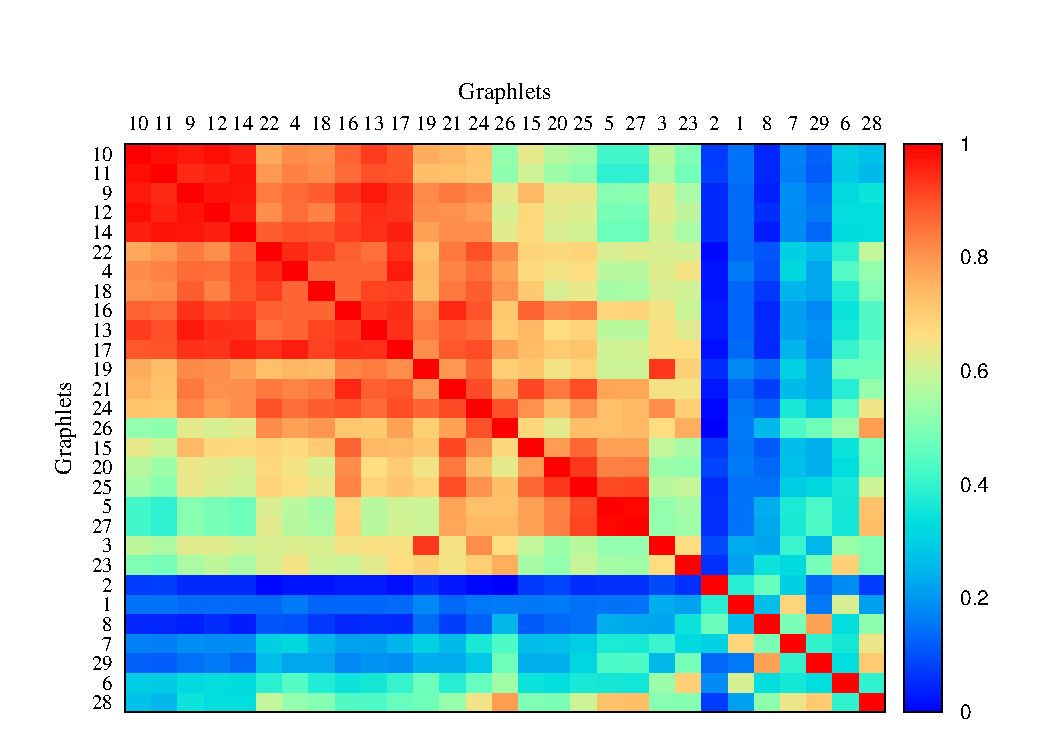
\includegraphics[scale=1.0]{../code/final_results_norm1/trade_2010_thresholded/heatmap_pearsons_hclust_trade_2010_thresholded2.pdf}}
  \caption[Pearson's GCV correlation matrix for the 2010 WTN using the normalised GCV]{Pearson's GCV correlation matrix for the 2010 WTN using the normalised GCV. The heat map is normalised only with feature scaling.}
  \label{fig:trade_norm1}
\end{figure}


% can also use \item[\textbf{A}]
Figure \ref{fig:trade_norm1} shows the Pearson's correlation matrix on the 2010 WTN that is calculated using the normalised GCV signature. We can observe several clusters of graphlets that have been formed along the diagonal:
\begin{itemize}
 \item \textbf{A}: Cluster made of graphlets \{10,11,9,12,14\}. These are all sparse graphlets that have 4 or 5 nodes.
 \item \textbf{B}: A slightly similar cluster that is also correlated with the one above is \{22,4,18,16,13,17\}. These graphlets all contain a $C_4$ as a subgraph.
 \item \textbf{C}: Another cluster is formed by graphlets \{5,25,27\}. These graphlets all contain a cycle of length 4 ($S_4$).  
\end{itemize}

However, we also notice that this time the cliques \{2,8,29\} do not cluster together. Cliques used to cluster together when using the un-normalised GCV signature (see figure \ref{fig:trade_heatmap}). We do not have a clear explanation for this behaviour and further research needs to be done into this. 

\subsection{Normalised GCV - Canonical Correlation Analysis}
\label{cca_trade_norm1}

After finding out which graphlets cluster together, we run Canonical Correlation Analysis using the same methodology described in section \ref{sec:cca_orig}, this time using the normalised GCV signature. Figure \ref{fig:all_trade_cca_black} shows the results of the CCA, while the supplementary table with all the correlations can be found in the appendix figure \ref{all_trade_thresh_cca}. The correlation is high $\rho = 0.94$ and the p-value is 0.0, suggesting that the result is statistically significant. 



% \rowcolors{1}{}

%                           red        green
% \definecolor{cca73p}{rgb}{0.13,0.87,0} % med blue
% \definecolor{cca29p}{rgb}{0.35,0.65,0} % med blue
% \definecolor{cca10n}{rgb}{0.55,0.45,0} % med blue
% % \definecolor{cca-26}{rgb}{1+0.26,0.29,0} % med blue
% 
% \definecolor{cca80n}{rgb}{0.90,0.10,0}



\newcommand{\ccaIndicatorsTradeNorm}{
  \begin{tabular}{r}
  \cellcolor{black}\textcolor{ccacol1}{POP}\\
  \cellcolor{black}\textcolor{ccacol1}{LE}\\
  \cellcolor{black}\textcolor{ccacol2}{KI}\\
  \cellcolor{black}\textcolor{ccacol2}{RGDPCH x POP}\\
  \cellcolor{black}\textcolor{ccacol2}{RGDPL x POP}\\
  \cellcolor{black}\textcolor{ccacol2}{RGDPL2 x POP}\\
  \cellcolor{black}\textcolor{ccacol2}{KG x RGDPL x POP}\\
  \cellcolor{black}\textcolor{ccacol2}{KC x RGDPL x POP}\\
  \cellcolor{black}\textcolor{ccacol3}{KC x RGDPL}\\
  \cellcolor{black}\textcolor{ccacol4}{XRAT}\\
  \cellcolor{black}\textcolor{ccacol4}{RGDPCH}\\
  \cellcolor{black}\textcolor{ccacol4}{RGDPL}\\
  \cellcolor{black}\textcolor{ccacol4}{RGDPL2}\\
  \cellcolor{black}\textcolor{ccacol4}{KG x RGDPL}\\
  \cellcolor{black}\textcolor{ccacol4}{KI x RGDPL}\\
  \cellcolor{black}\textcolor{ccacol4}{KC}\\
  \cellcolor{black}\textcolor{ccacol5}{KI}\\
  \cellcolor{black}\textcolor{ccacol5}{BCA per RGDPL}\\
  \cellcolor{black}\textcolor{ccacol5}{KG}\\
  \cellcolor{black}\textcolor{ccacol5}{BCA}\\
  \cellcolor{black}\textcolor{ccacol6}{OPENK}
  \end{tabular}

}


\begin{figure}[H]
  \centering
    \begin{tikzpicture}[scale=\ccafigscale,show background rectangle, 
  background rectangle/.style={fill=black},
  color=white,help lines/.style={color=lightgray,line width=0.2pt},post/.style={->,shorten >=1pt,>=stealth',thick}]

    \node[upper left,inner sep=0,scale=\ccafigscale] (indicators) at (-2.0,0) {\ccaIndicatorsTradeNorm};	
    \shade[top color=green,bottom color=yellow] (4,0) rectangle (4.5,5);
    \shade[top color=yellow,bottom color=red] (4,-5) rectangle (4.5,0);
    \node[upper left,inner sep=0] (dummy) at (13.0,4) {}; % for extending the black bounding box
    \node[upper left,inner sep=0] (corr_text) at (4.25,-6.0) {Correlation};
    \node[upper left,inner sep=0,red] (corr_text) at (4.25,-5.5) {-1};
    \node[upper left,inner sep=0, green] (corr_text) at (4.25,5.5) {1};
    \node[upper left,inner sep=0] (corr_text) at (4.75,0) {0};
    
    \node[upper left,inner sep=0,scale=\ccafigscale] (g12) at (7.5,4.0) {\gtwelvecca{ccacol1}};
    \node[upper left,inner sep=0,scale=\ccafigscale] (g10) at (10.5,2.5) {\gtencca{ccacol1}};
    \node[upper left,inner sep=0,scale=\ccafigscale] (g14) at (7.5,1.0) {\gfourteencca{ccacol1}};
    \node[upper left,inner sep=0,scale=\ccafigscale] (g2) at (10.5,-1.0) {\gtwocca{ccacol8}};
    \node[upper left,inner sep=0,scale=\ccafigscale] (g29) at (7.5,-2.5) {\gtwentyninecca{ccacol8}};
    \node[upper left,inner sep=0,scale=\ccafigscale] (g8) at (10.5,-4.0) {\geightcca{ccacol8}};
    
    
%     \draw[line,color=ccacol1] (0,4.8) -| (3,5) -- (4.25,5); % top-left elem
%     \draw[line,color=ccacol1] (0,4.35) -| (2,3.9) -- (4.25,3.9); % next in line
    
    \draw[line,color=ccacol1] (0.00,4.80) -| (1.75,3.68) -- (4.00,3.68);
    \draw[line,color=ccacol1] (0.00,4.33) -| (1.49,3.58) -- (4.00,3.58);
    \draw[line,color=ccacol1] (0.00,3.85) -| (1.37,3.30) -- (4.00,3.30);
    \draw[line,color=ccacol1] (0.00,3.38) -| (1.07,3.27) -- (4.00,3.27);
    \draw[line,color=ccacol1] (0.00,2.90) -| (1.25,3.27) -- (4.00,3.27);
    \draw[line,color=ccacol1] (0.00,2.42) -| (1.56,3.26) -- (4.00,3.26);
    \draw[line,color=ccacol1] (0.00,1.95) -| (1.84,3.21) -- (4.00,3.21);
    \draw[line,color=ccacol1] (0.00,1.48) -| (2.13,3.17) -- (4.00,3.17);
    \draw[line,color=ccacol3] (0.00,1.00) -| (1.31,1.46) -- (4.00,1.46);
    \draw[line,color=ccacol4] (0.00,0.53) -| (1.22,0.85) -- (4.00,0.85);
    \draw[line,color=ccacol4] (0.00,0.05) -| (1.50,0.80) -- (4.00,0.80);
    \draw[line,color=ccacol4] (0.00,-0.42) -| (1.82,0.80) -- (4.00,0.80);
    \draw[line,color=ccacol4] (0.00,-0.90) -| (2.13,0.80) -- (4.00,0.80);
    \draw[line,color=ccacol4] (0.00,-1.38) -| (2.30,0.79) -- (4.00,0.79);
    \draw[line,color=ccacol4] (0.00,-1.85) -| (2.58,0.52) -- (4.00,0.52);
    \draw[line,color=ccacol4] (0.00,-2.33) -| (2.68,0.43) -- (4.00,0.43);
    \draw[line,color=ccacol5] (0.00,-2.80) -| (2.77,-0.08) -- (4.00,-0.08);
    \draw[line,color=ccacol5] (0.00,-3.27) -| (2.92,-0.55) -- (4.00,-0.55);
    \draw[line,color=ccacol5] (0.00,-3.75) -| (3.07,-0.64) -- (4.00,-0.64);
    \draw[line,color=ccacol5] (0.00,-4.23) -| (3.32,-0.75) -- (4.00,-0.75);
    \draw[line,color=ccacol6] (0.00,-4.70) -| (3.55,-1.33) -- (4.00,-1.33);

    
    
    \draw[line,color=ccacol1] (g12) -| (5.5,4.5) -- (4.5,4.5);
    \draw[line,color=ccacol1] (g10) -| (5.3,4.47) -- (4.5,4.47);
    \draw[line,color=ccacol1] (g14) -| (5.1,4.43) -- (4.5,4.43);

    \draw[line,color=ccacol8] (g2) -| (5.3,-2.5) -- (4.5,-2.5);
    \draw[line,color=ccacol8] (g29) -| (5.5,-3) -- (4.5,-3);
    \draw[line,color=ccacol8] (g8) -| (5.1,-3.5) -- (4.5,-3.5);
    
    \end{tikzpicture}
    \caption[CCA - World Trade networks - normalised GCV - Picture version]{CCA between economic indicators and the normalised GCV signature. Only the graphlets that show the strongest respectively weakest correlations are shown. One can notice that graphlets \{12,10,14\} are relatively sparse, while graphlets \{2,29,8\} are dense, being cliques. The sparse graphlets are correlated with the good economic indicators (in green) such as Population (POP), Level of Employment (LE) and GDP per Capita (RGDPL), while dense graphlets are correlated with bad indicators (in red) such as the Balance of Current Account (BCA). The canonical correlation $\rho = 0.94$ and the p-value is smaller than 0.0001, suggesting that the result is statistically significant.}
    \label{fig:all_trade_cca_black}	
\end{figure}


The good indicators such as population (POP), level of employment (LE) and GDP per capita (RGDPL) are positively correlated with the graphlets \{12,10,14,17,9, \dots \}\footnote{The CCA figure \ref{fig:all_trade_cca_black} only shows the graphlets that have the strongest and weakest cross-loadings. See figure \ref{all_trade_thresh_cca} in the appendix for a list of cross-loadings for all the graphlets and economic indicators.}. On the other hand, the bad indicators such as the balance of current account (BCA) correlate positively with graphlets \{8,29,2,7,1,28\}. Graphlets \{10,12,14,9\} on the positive side of the spectrum have also clustered together in the Pearson's correlation matrix (section \ref{sec:trade_pears_norm1}). We first notice that graphlets \{8,29,2,7,1,28\} represent cliques \{8,29,2\} or almost cliques \{7,1,28\}. Since these graphlets are very densely connected, this suggests that the trading partners of small and poor countries are trading heavily with each other or form highly connected 
clusters. As a result, we deduce that \emph{the majority of the trading partners of small and poor countries are the big and rich countries that are always trading heavily with each other}. 

This theory seems to be confirmed by taking a few small and poor countries and looking at their trading partners. Note that since the network has only 119 countries, the poorest countries from Africa or South Asia have already been filtered out.\footnote{This is the case because the network has been thresholded at an 85\% level. See section \ref{sec:trade_bck} for more details.} Therefore, let us consider Morocco a small and poor country relative to the others, although in reality it considered to have a medium level of development. Morocco's main trading partners are: Saudi Arabia, China, France, USA, Spain, Germany and Italy. These countries are big and rich and every single pair of them clearly trade with each other. Similar results have been observed for other countries such as Uruguay. Moreover, all of Morocco's trading partners are part of G20, a club of big and wealthy countries that collaborate with each other on economic matters. This leads us to a second theory: \emph{since the trading 
partners of a small and poor country form highly connected clusters, these clusters represent big and rich economic groups such as G8, G20, OECD\footnote{Organisation for Economic Co-operation and Development} or Paris-club\footnote{A group of countries that provide debt relief and debt restructuring to indebted countries and their creditors.}}. This theory can be validated by selecting a few countries and looking at their neighbours. For example, the biggest trading partners of Tunisia are Germany, France and Italy, all part of G8, G20, OECD and Paris-club. 

Regarding the first group of graphlets (i.e.\ \{12,10,14, \dots \}), we notice that all of them are sparse graphlets that contain relatively few edges. Having the sparse graphlets at one end of the spectrum and the dense graphlets at the other suggests that the graphlets are roughly ordered according to their density. Therefore, CCA shows that the sparse graphlets correlate with the good indicators such as population (POP), level of employment (LE) and GDP per capita (RGDPL) while dense graphlets correlate with bad indicators such as the balance of current account (BCA).

Now that we now know to interpret the positively weighted part of the graphlet vector as sparse graphlets, canonical correlation tells us that the trading partners of big and wealthy countries have a lot of sparse graphlets in their neighbourhood. The economic reason for this is because \emph{big and rich countries like USA, China, Russia are trading with a lot of small, isolated countries which in turn do not trade with each other}. This theory is supported by a closer analysis with Cytoscape\footnote{A network analysis software that can provide useful statistics of the network data.}. Using this software we found that the clustering coefficient of a country is inversely correlated with the wealth and size of that country, suggesting that big and rich countries indeed have a relatively sparse neighbourhood.


\subsection{Normalised GCV - Correlation matrix change during 1962--2010}
\label{rev_trade_change}

% Put them when the report is ready
% gcv offset: -1   Spearman's rank coefficient: corr: 0.340675635498    p_value: 0.0191171684701

We also calculated the changes in Pearson's correlation matrix using the normalised GCV for the WTNs over the period 1962--2010. The results are plotted in figure \ref{change_over_time_norm1} along with the changes in Crude Oil price. For this experiment we follow the same methodology as in section \ref{trade_change_orig}. We find that for the normalised GCV, the best results are obtained when the GCV vector is shifted with -1 year and yields a positive correlation $\rho = 0.34$ and a p-value of $p = 0.01$. These results are in contrast to the ones obtained using the original GCV signature in section \ref{trade_change_orig} and at the moment we cannot give a reason why this is happening. Since the best correlation is obtained when the GCV vector is shifted with -1, this again suggests that the changes in the network structure might cause the changes in the price of Crude Oil.

\begin{figure}[H]
  \centering
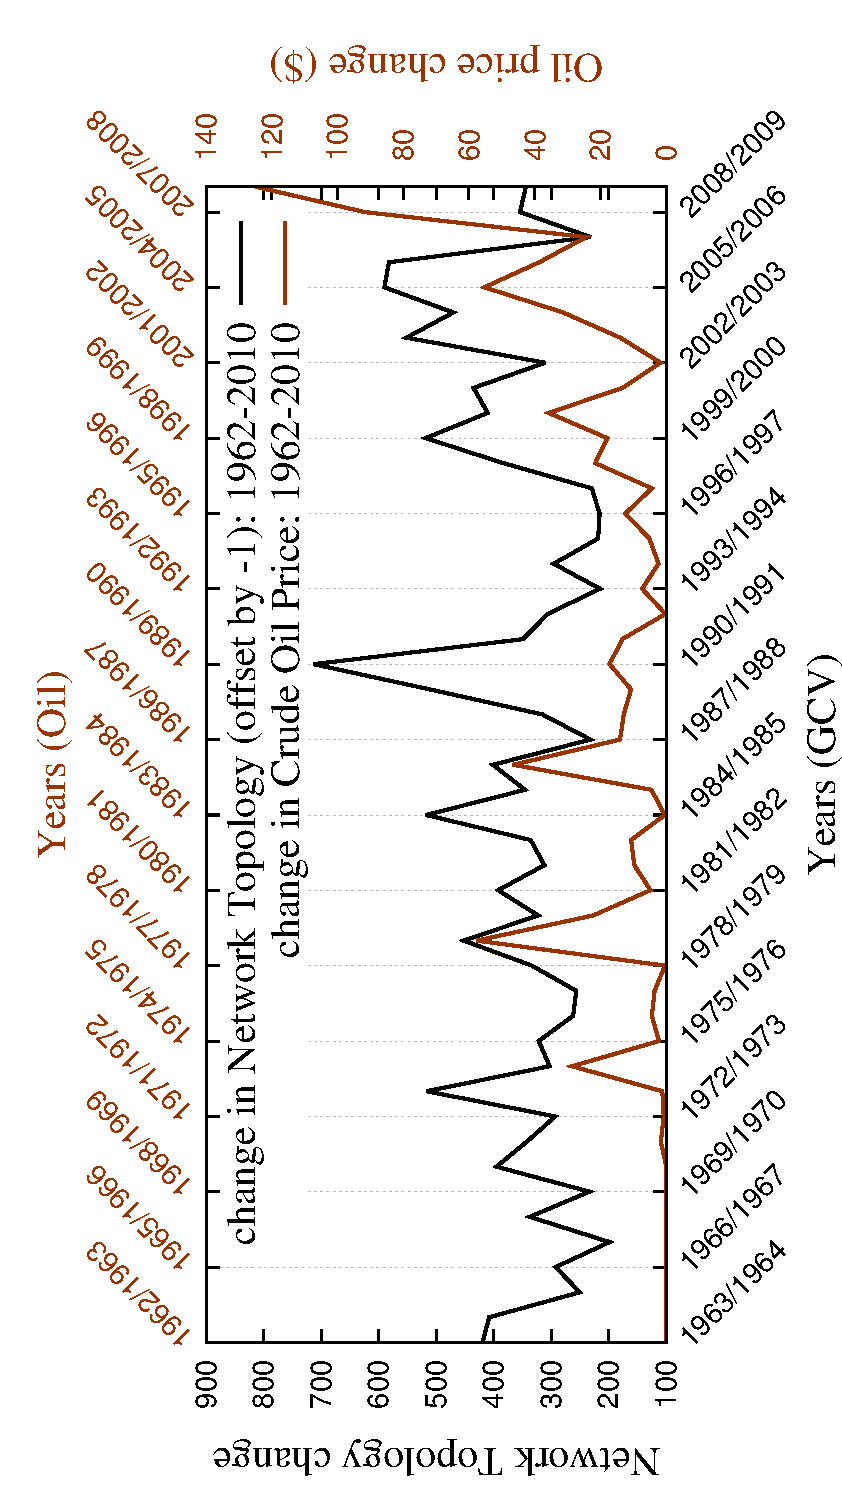
\includegraphics[angle=-90,scale=0.6]{../code/final_results_norm1/all_trade_thresh/change_over_time2}
\caption[Change in WTN topology - normalised GCV]{Change in WTN topology (as measured by the normalised GCV correlation matrix) versus change in crude oil price. The two plots are positively correlated, having a Spearman's rank correlation coefficient of 0.34 and p-value of 0.01. The best correlation coefficient is obtained when the change in network topology is shifted by -1 years. The top and left axis tics correspond to the Oil curve, while the bottom and the left axis tics correspond to the network topology curve.}
\label{change_over_time_norm1}
\end{figure}

There are several major economic and social events that have clearly affected the WTN structure. The 1970s were marked by two energy crises (1973 and 1979) that explain the two small peaks in both the topology change but also in the oil price change. Afterwards, the 1983/1984 peak in network topology change might have been caused by the early 1980s recession, which affected most of the developed world. A revival of neoliberalist economic policies around the world occurred in this period which led to reduced government intervention, lower taxes and deregulation. The peak in 1989 might be explained by the fall of communist/socialist governments in Russia, Eastern Europe and around the world accompanied by a fall in heavy industries and increased trade openness. These events have been accompanied by changes in government for some former left-wing or right-wing countries such as Russia, Poland, Chile and South Africa.

The early 1990s appear as a period of relatively low changes in oil and network topology, which reflects the overall economic stability at that time. However, bigger changes are noticed in the late 1990s, possibly started by the 1997 Asian financial crisis. By the 2000s, even bigger changes can be observed in the network topology plot that were caused by the commodities boom and rising oil prices and inflation. 

\subsection{Trade partners sparsity index}
\label{sec:sparsity_index}

Using a combination of graphlet frequencies that are part of the GCV, we are now interested to create an index that is positively correlated with the good indicators from section \ref{cca_trade_norm1} such as GDP per Capita (RGDPL) or Level of Employment (LE). Therefore, we take the three graphlets that have the highest correlation with the economic indicators variate \{12,10,14\} and the three that have the lowest correlation \{8,29,2\} (see figure \ref{all_trade_thresh_cca}). Multiplying each of these by their respective CCA cross-loading and summing up the results gives us a \emph{trading partner sparsity index}. The index $T$ can formally be defined as:

$$ T = w_{12}F_{12} + w_{10}F_{10} + w_{14}F_{14} + w_{8}F_{8} + w_{29}F_{29} + w_{2}F_{2}$$
where $F_i$, $w_i$ are the frequency respectively the canonical cross-loading of $G_i$. In order to compute the index, we use the cross-loadings obtained from CCA in figure \ref{all_trade_thresh_cca}.

This index can be calculated for every country and for every year and can have both positive and negative values. It gives a measure of the sparsity of the network of the trading partners: the higher the value the sparser the neighbourhood, because the sparse graphlets have positive weights while the dense graphlets have negative weights. CCA has shown us that for a certain country a network of trading partners that 
has sparse graphlets indicates a healthy economy, so we expect the \emph{trading partner sparsity index} to be high for big and wealthy countries and low for small and poor countries. We also expect the index to fluctuate during periods of economic uncertainty.

\begin{figure}[H]
  \centering
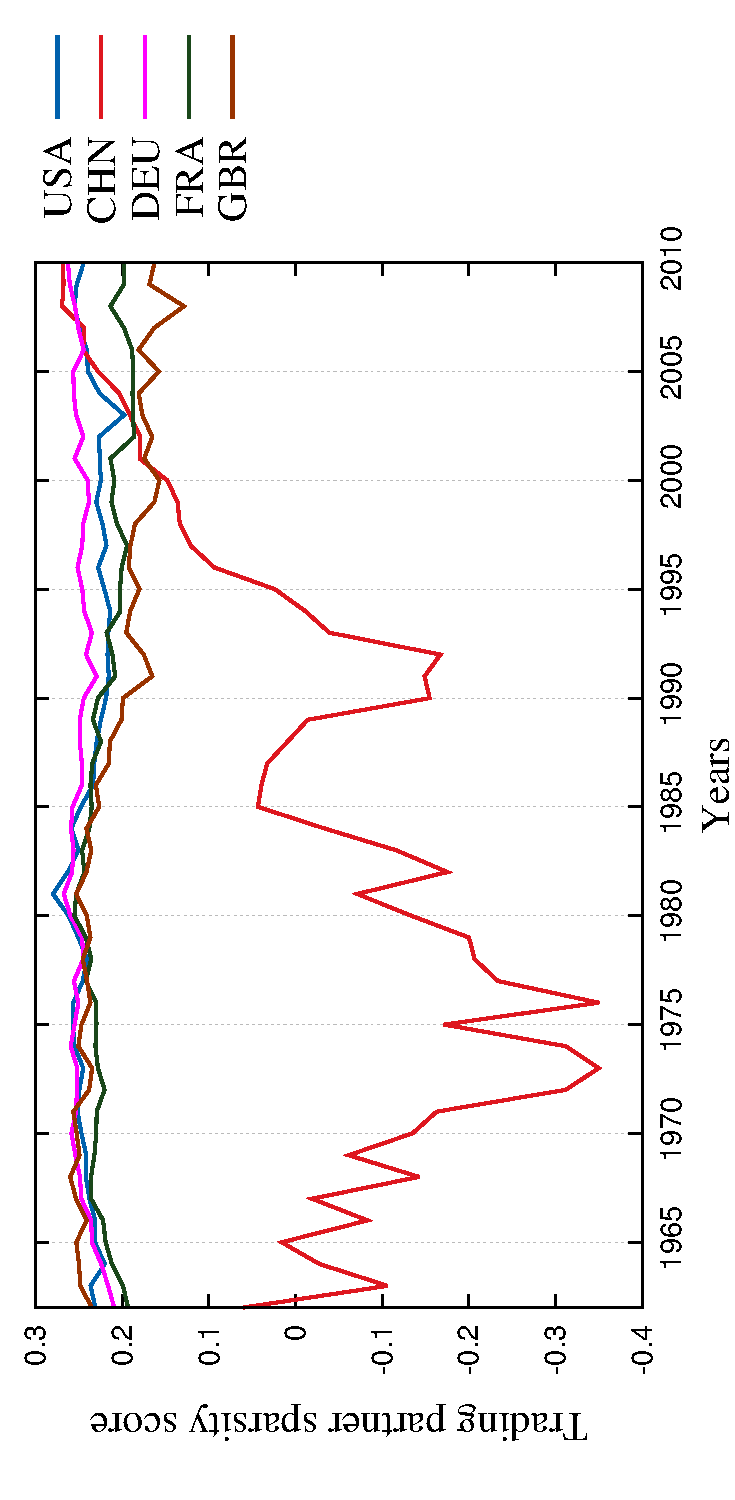
\includegraphics[angle=-90,scale=0.6]{../code/extra_results/trading_partner_density/scores/g72.pdf}
\caption[Trading partners sparsity index -- United States (USA), China (CHN), Germany (DEU), France(FRA) and the United Kingdom (GBR)]{Trading partners sparsity index measured for 5 big economies: United States (USA), China (CHN), Germany (DEU), France(FRA) and the United Kingdom (GBR). The index for US, Germany, France and the UK is approximately flat over the 49-year period. However, the index of China has a downward trend over the time period 1963--1973 due to Mao Zedong's policies that harmed the economy of the country. However, the period after 1975 shows a surge that was boosted by economic reforms and growth. There is one exception in 1990--1992 right after the Fall of Communism in Eastern Europe, a global event that affected a socialist country such as China.}
\label{g7_sparsity_index}
\end{figure}

Figure \ref{g7_sparsity_index} shows the \emph{trading partners sparsity index} for several influential countries: United States (USA), China (CHN), Germany (DEU), France(FRA) and the United Kingdom (GBR). Throughout the 1965--2010 period, the corresponding index for the United States, Germany, France and the United Kingdom has been approximately flat, having a value of 0.2. Some small variation can be seen starting from 1990, with Germany and the United States having a slightly bigger index than France and the United Kingdom. Furthermore, for these four countries we don't observe any shocks during economic crises. On the other hand, China suffers a decrease in the trading partners sparsity index during 1965--1976, due to Mao Zedong's Cultural Revolution that resulted in a period of economic decline. However, the index increases again during 1976--1985, probably due to economic reforms that were initiated by Deng Xiaoping which helped revive the economy. Another low point is noticed in 1990--1992 right at 
the Fall of Communism in USSR and Eastern Europe, a global event that deeply affected a socialist state such as China.

\begin{figure}[H]
  \centering
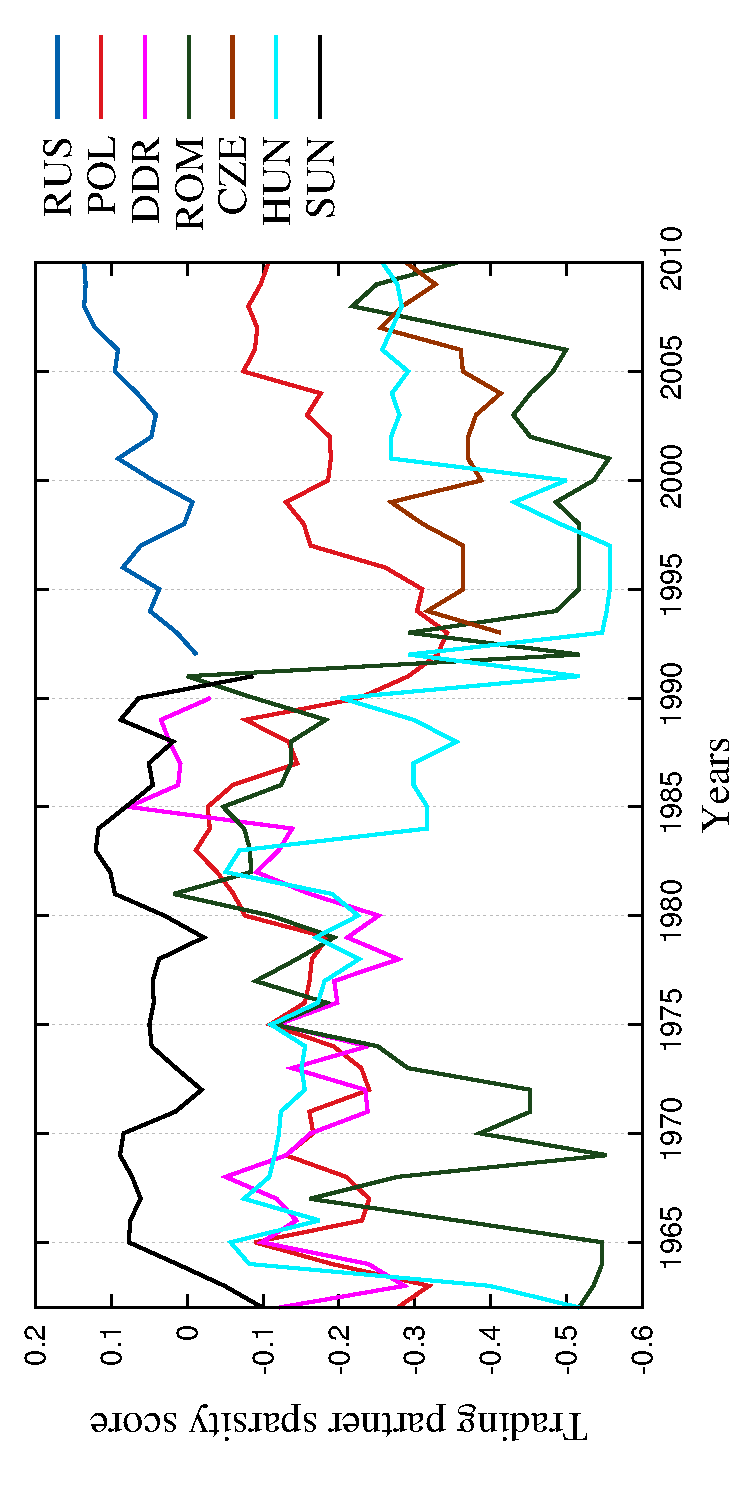
\includegraphics[angle=-90,scale=0.6]{../code/extra_results/trading_partner_density/scores/eastern_europe2.pdf}
\caption[Trading partners sparsity index -- Russia (RUS), Poland (POL), East Germany (DDR), Romania (ROM), Czech Republic (CZE), Hungary (HUN) and the USSR (SUN)]{Trading partners sparsity index measured for countries from Eastern Europe: Russia (RUS), Poland (POL), East Germany (DDR), Romania (ROM), Czech Republic (CZE), Hungary (HUN) and the USSR (SUN). Most of the countries show a drop in the index after 1990 because of the Fall of Communism and the economic restructuring that took place at that time.}
\label{eastern_europe_sparsity_index}
\end{figure}

Figure \ref{eastern_europe_sparsity_index} shows the \emph{trading partners sparsity index} for several countries in Eastern Europe: Russia (RUS), Poland (POL), East Germany (DDR), Romania (ROM), Czech Republic (CZE), Hungary (HUN) and the USSR (SUN). In the period leading to 1990, the USSR had the highest index since it was a world superpower, while it's satellite states had a lower index. However, the Revolutions in December 1989 in Eastern Europe led to a large drop in the \emph{trading partners sparsity index} for all these countries, a fact that is reflected by the economic situation at that time: unemployment skyrocketed and living standards fell considerably. It took some countries such as Poland of Hungary around approximately 10--15 years to reach the pre-revolutions level in the \emph{trading partners sparsity index}.

\begin{figure}[H]
  \centering
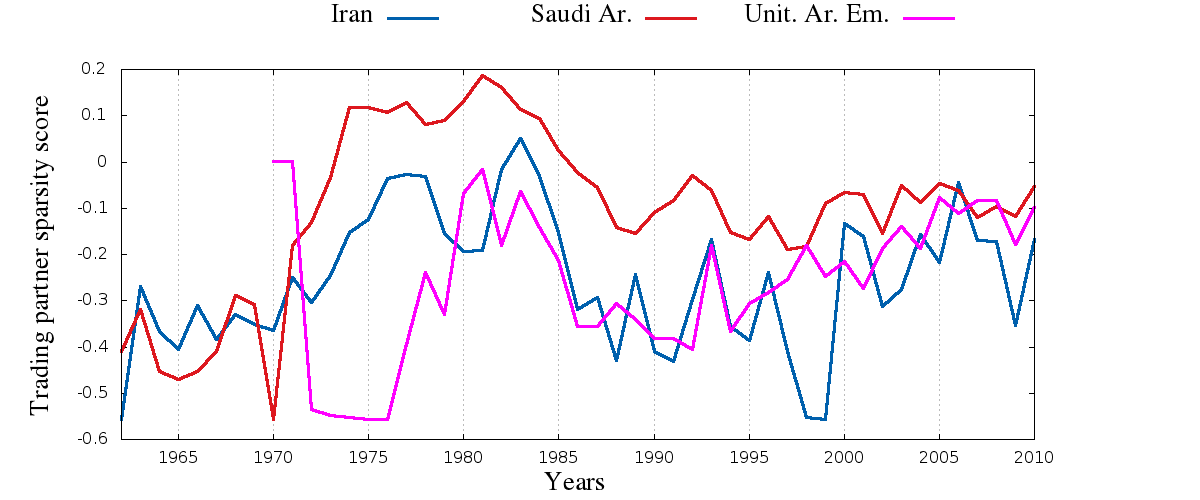
\includegraphics[angle=-90,scale=0.6]
{../code/extra_results/trading_partner_density/scores/opec2}
\caption[Trading partners sparsity index -- Iran (IRN), Saudi Arabia (SAU) and United Arab Emirates (ARE)]{Trading partners sparsity index measured for 3 OPEC members: Iran (IRN), Saudi Arabia (SAU) and United Arab Emirates (ARE). The rise in petroleum prices and the Oil crisis in 1973 has led to a surge in the index for Saudi Arabia and Iran. Moreover, the Oil crisis of 1979 has also led to an increase in United Arab Emirate's index. However, the 1980s Oil glut that was caused by a serious surplus of oil had detrimental effects on all OPEC members, which is reflected in the drop of their trading partners density index.}
\label{opec_sparsity_index}
\end{figure}

Figure \ref{opec_sparsity_index} shows the \emph{trading partners sparsity index} for three main OPEC members: Iran, Saudi Arabia and United Arab Emirates. For Saudi Arabia and Iran, the rise in petroleum prices in 1970s led to a surge in it's index. However, during the 1980s the oil glut that was caused by a serious surplus of crude oil and a drop in demand had detrimental effects on all OPEC members, which are heavily dependent on the price of oil. It can also be noticed that the 1973 Oil Crisis has led to an increase in the index only for Saudi Arabia and Iran, while the 1979 Oil crisis has led to an increase in the index only for the United Arab Emirates.

\subsection{Case study: Saudi Arabia}
\label{case_study_saudi}
% norm1 GCV vector results

%gcv offset: -1   Spearman's rank coefficient: corr: -0.323529495316    p_value: 0.0265331450245
% offset 1 gives the best results .. tried [-2,-1,0,1,2]

% orig GCV results are all bad, even if offset by +- 0-2 years

As we have seen in previous sections, the GCV signature can indeed capture the changes in Crude Oil prices and correlate with key economic and social events around the world. In this section we are trying to apply the same analysis but on a smaller scale, at a country level. We have selected Saudi Arabia as a major oil-exporting country, whose economy is heavily dependent on the price of oil. We are trying to find the answer to the following questions:
\begin{itemize}
 \item Are the partners of Saudi Arabia affected by changes in Crude Oil price?
 \item Is the GCV of Saudi Arabia positively or negatively correlated with the Crude Oil Price?
\end{itemize}

Saudi Arabia is the world's largest oil-exporting economy and has the largest proven petroleum reserves. It is also a very influential member of the \emph{Organisation of the Petroleum Exporting Countries} (OPEC). It's main export partners are the United States, China and Japan, while it's main import partners are China, United States and South Korea. Around 90\% of it's exports consist of petroleum and related products. 

We therefore calculate the normalised GCV of Saudi Arabia for each year in the period 1962--2009. Afterwards, the change in GCV between every two consecutive years is calculated using the Euclidean distance between the two vectors. Results of the GCV change along with the Crude Oil price are plotted in figure \ref{saudi_oil}. The two plots are negatively correlated, having a Spearman's rank correlation coefficient of -0.32 with a p-value of 0.026, which resembles the results we got for the original GCV change for the overall trade network in section \ref{trade_change_orig}. First of all, it must be noted that since Saudi Arabia is an oil-exporting country, it benefits massively from a rise in oil prices. However, high oil prices on the energy markets lead to less demand for petrol and provides other oil-poor countries an incentive for developing alternative sources of energy. The fact that Saudi Arabia benefits from high oil prices might explain why the change in it's trading partner network topology is 
inversely correlated with oil price: when the price of oil is low, Saudi Arabia always looks for new export markets and thus has a move volatile network of trading partners. On the other hand, when the price of oil is high, it means that the demand is much higher than the supply available, so Saudi Arabian oil companies prefer to export to their old trading partners, since there is no need for extra contracts, negotiations and bureaucracy.

Figure \ref{saudi_oil} shows that big changes in the trading partners of Saudi Arabia occurred between 1968/1969 and 1969/1970, which subsumed shortly afterwards. These might be explained as a consequence of the 1967 Oil Embargo, when Saudi Arabia and several Middle Eastern countries limited or completely stopped their oil supplies to Western countries such as the USA, UK and other European states. The result was that Saudi Arabia had to look for different export partners and that led to a change in its trading partner structure.

This experiment has also been run using the un-normalised GCV change, but it hasn't yielded a good correlation between the GCV change and the change in crude oil price. The associated p-value was also high, meaning that the result was not statistically significant. A plot and the equivalent results are given in figure \ref{saudi_oil_orig} in the appendix.

\begin{figure}[H]
  \centering
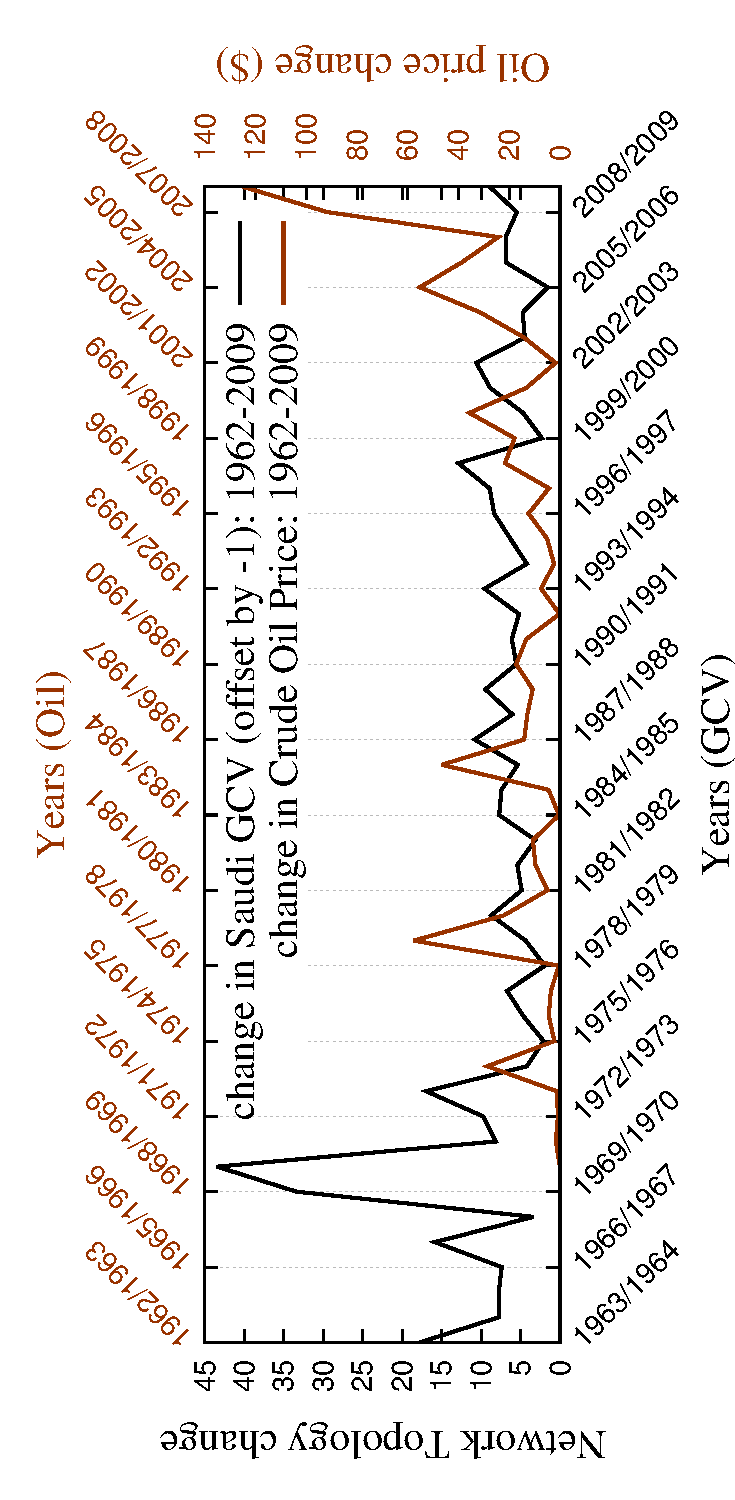
\includegraphics[angle=-90,scale=0.6]
{../code/extra_results/saudi_oil/saudi_norm1_gcv_oil2}
\caption[The change in the GCV of Saudi Arabia along with the change in Crude Oil price.]{The change in the GCV of Saudi Arabia along with the change in Crude Oil price. The two plots are negatively correlated, having a Spearman's rank correlation coefficient of -0.32 with a p-value of 0.026. This correlation is obtained when the vector of changes in Saudi GCV is shifted by -1. Top and left axis tics correspond to the Oil curve, while the bottom and the right axis tics correspond to the Saudi GCV curve.}
\label{saudi_oil}
\end{figure}


%cca_oil/CCA_out/saudi_oil.txt

In order to find out how each of the individual elements of the GCV vector are influenced by the oil price, we apply Canonical Correlation between the GCV of Saudi Arabia and the Crude Oil price index. However, this proves to be problematic since we only have 49 samples to run the CCA on, one for every year during 1962--2010\footnote{In previous CCA experiments, we used all country-year pairs that gave us in total around $119 * 29 = 3451$ samples, where $119$ is the average number of countries in the network and $29$ is the number of years CCA was run on (period 1980-2010). The reason CCA was run from 1980 is because we did not have data for the economic indicators prior to 1980.}. On the other hand, there are $29 (\text{GCV}) + 1(\text{Oil Price}) = 30$ parameters that need to be estimated. This could easily overfit or yield singularities in our algorithm. Therefore, we trim down the GCV vector to only contain the essential graphlets 1-8, discarding all the 5-node graphlets. The final CCA variates  are as 
follows:
\begin{itemize}
 \item[X] - short 8-element GCV of Saudi Arabia that only contains the essential graphlets (i.e.\ $G_1-G_8$)
 \item[Y] - a single-element vector containing the Oil price 
\end{itemize}

Results for the CCA analysis are shown in figure \ref{saudi_oil_cca}. It is shown that graphlet $G_3$ correlates positively with the increase in Oil price, while graphlets \{1,2,8\} correlate negatively. One property that separates the two ends of the graphlet spectrum is their density. Graphlet $G_3$ is a sparse graphlet, while graphlets \{1,2,8\} are dense graphlets having a density of at least 0.66. 

Using the results we got earlier from section \ref{cca_trade_norm1}, we know that sparse graphlets correlate with good economic indicators such as GDP per Capita (RGDPL), while dense graphlets correlate with bad economic indicators such as Balance of Current Account (BCA). Using this observation and the fact that sparse graphlets correlate positively with the oil price and dense graphlets vice versa, we can conclude that for Saudi Arabia the good economic indicators such as GDP per Capita, a result of a healthy economy, must correlate with the Oil price\footnote{if the correlation of XY is strictly positive and the correlation of YZ is likewise, then the correlation of X and Z is not necessarily strictly positive. This is however the case if the correlations of XY respectively YZ are close to 1 \cite{langford2001property}.}. This is confirmed by the fact that Saudi Arabia is an Oil-exporting economy, and it's GDP per Capita has been shown to strongly correlate with the Oil price \cite{
lescaroux2008influence}. We expect similar behaviour for other oil-exporting economies such as Libya, Venezuela, Qatar or Russia.

\begin{figure}[H]
\centering
\begin{tabular}{ c c | c c }
  \multicolumn{2}{c}{Canonical Correlation} &  \multicolumn{2}{c}{0.82353} \\
  \multicolumn{2}{c}{p-value} &  \multicolumn{2}{c}{0.00000} \\
  \hline
  \multicolumn{2}{c}{X variate} & \multicolumn{2}{c}{Y variate}\\
  \hline
 G3 & 0.49265 &  Crude Oil price & 0.83032\\
 G6 & 0.09838 &  & \\
 G4 & 0.05294 &  & \\
 G5 & 0.03942 &  & \\
 G7 & -0.23884 &  & \\
 G8 & -0.46603 &  & \\
 G2 & -0.50725 &  & \\
 G1 & -0.52241 &  & \\
\end{tabular}
\caption[Canonical Correlation Analysis between the short GCV vector of Saudi Arabia and the price of Crude Oil.]{Canonical Correlation Analysis between the short GCV vector of Saudi Arabia and the price of Crude Oil. Only the short GCV-8 vector has been used because of the lack of samples. The results show that graphlet $G_3$ is has a strong positive correlation with the price of Crude Oil, while graphlets \{1,2,8,7\} have a negative correlation. This suggests that when the price of Oil is high, the trading partners of Saudi Arabia tend to form paths of 4 nodes ($P_4$). On the other hand, when the price of Oil is low, the trading partner network of Saudi Arabia tends to cluster (\{1,2,8,7\} are dense graphlets with a density of at least 0.66). This might be explained by the fact that when the price of Oil is high, Saudi Arabia starts new trading partnerships with isolated countries that are not part of a clustered network.}
\label{saudi_oil_cca}
\end{figure}


\section{Protein-protein Interaction Networks}
\label{ppi_res_heatmaps}

In this section we apply our methodology for various PPI Networks. For more background information about how these networks are built and their properties, see section \ref{sec:ppi_bck}. We now present the Pearson's correlation matrix for a Human PPI network and Canonical Correlation Analysis results for six different Human and Yeast PPI networks using two annotation files: Boone's and von Mering's (see annotation descriptions in section \ref{sec:ppi_bck}). In short, the heat map of the Pearson's GCV correlation matrix did not give us any useful information, since graphlets formed faint clusters. However, the CCA results have helped us get some interesting insights into the interactions of the proteins present in these networks. 

\subsection{Analysis of Pearson's GCV Correlation Matrix}

\begin{figure}
  \centering
  \hbox{\hspace{-1cm}
  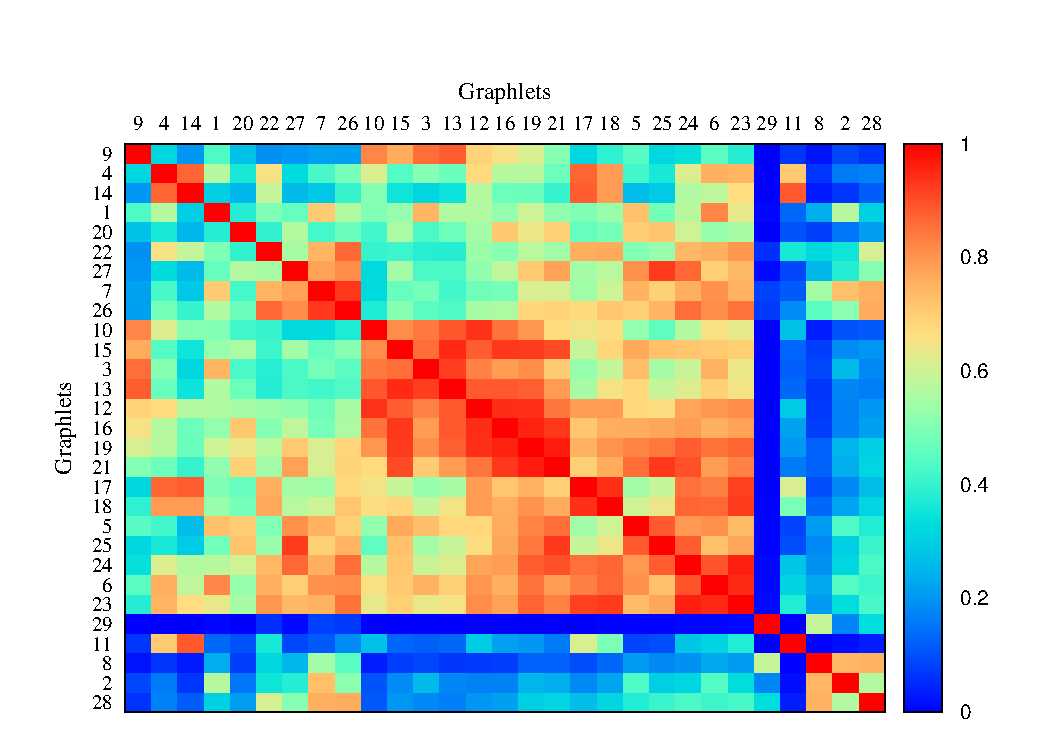
\includegraphics[scale=1.0]
  {../code/final_results/human_ppi/heatmap_pearsons_hclust_human_ppi-poly-42.pdf}}
  \caption[Heat map for the Pearson's GCV correlation matrix of the Human PPI network]{Heat map for the Pearson's GCV correlation matrix of the Human PPI network. The heat map has been first normalised with feature scaling and a $4^{th}$ degree polynomial and then hierarchically clustered.}
  \label{fig:human_ppi}
\end{figure}



The heat map from figure \ref{fig:human_ppi} represents the Pearsons's correlation heat map for the Human PPI 
network. It was first normalised with a simple feature scaling and then with a $4^{th}$ degree polynomial\footnote{Other polynomial functions have also been tested, but the $4^{th}$ degree polynomial offers the best results.}, because the original correlation matrix yielded correlations that were too strong\footnote{Having all correlations close to 1 made the identification of clusters impossible}. There are a few faint clusters formed on the diagonal:
\begin{itemize}
 \item \{10,15,3,13,12,16,19 and 21\}. These graphlets all contain a $P_4$\footnote{Path on 4 nodes, graphlet $G_3$}.  
 \item \{7,26\} contain a $G_7$.
 \item \{4,14\} contain a $G_4$.
 \item \{17,18\} contain 2 $G_2$'s (triangles).
 \item \{5,25\} contain a $G_5$.
 \item \{24,6,23\} contain a $G_6$.
\end{itemize}

The lack of clear graphlet clusters in the Human PPI is something that we cannot 
explain at the current time. Because of this, it has not been possible for us to get any actual insights from the Human PPI correlation matrix. Other human and yeast PPI networks have yielded similar results. Further research needs to be done into this area in order to explain the lack of graphlet clustering.

\subsection{Canonical Correlation Analysis}


The next step after the Pearson's GCV correlation matrix is to run CCA on the PPI network. We set the $X$ variate to be the GCV and the $Y$ variate to be a vector of values of Boone's annotation. For setting up the $Y$ variate, we label each protein with a vector of binary entries, where the $i^{th}$ entry is as follows:

\rowcolors{1}{}{}
$$ Y_i = \begin{cases} 1, & \mbox{if the protein is annotated with the } i^{th}\mbox{ annotation} \\ 0, & \mbox{otherwise} \end{cases}$$

Since each protein had only one annotation, each sample from $Y$ only contained one non-null entry. The results of the CCA on this network were unfortunately not good, since the correlation is low and the p-value is above 0.05, suggesting that the correlation is not statistically significant. In the next section we will explain the subsequent experiments that have been performed on other PPI networks.

\subsection{Results for other PPI networks}
\label{sec:cca_ppi_intro}

\subsection*{The 17 experiments}


Since the CCA applied to the Human PPI network didn't give us any meaningful information, we thought of exhaustively running it on several types of Human and Yeast PPI networks. We ran the same process on 5 other Human PPI networks with Boone's annotation file and on 6 Yeast networks using the two different annotation files: von Mering's and Boone's (see section \ref{ppi_annotations}). For these experiments we have also used high-confidence networks, which contain only protein interactions that have been confirmed by two independent sources. The networks analysed are as follows:
\begin{itemize}
 \item 5 Human networks
 \begin{itemize}
    \item A high-quality Human PPI network determined by Stitch-seq protocol \cite{yu2011next}, CCA results are not statistically significant.\footnote{In this subsection by statistically significant we mean that either the p-value was above 0.05 or the total correlation was below 0.2}
    \item Two networks from I2D, a database of PPI networks maintained by Jurisca lab \cite{brown2007unequal} at Ontario Cancer Institute:
    \begin{itemize}
      \item Full version, CCA results are not statistically significant.
      \item High-confidence version, CCA results are not statistically significant.
    \end{itemize}
    \item Two networks from BioGRID: 
    \begin{itemize}
      \item Full version, CCA results are not statistically significant.
      \item High-confidence version, CCA results are not statistically significant.
    \end{itemize}
  \end{itemize}
 \item 6 Yeast networks x 2 annotation files
  \begin{itemize}
    \item A network obtained through \emph{affinity-purification mass spectroscopy} (AP-MS) by Collin's et al \cite{collins2007toward} - Co-complex membership associations, CCA results in figures  \ref{yeast_apms_collins_cca}, \ref{all_ppi12}
    \item A genetic network from BioGRID, CCA results in figures   \ref{all_ppi7}, \ref{all_ppi13}
    \item Literature-curated PPI network by Reguly et al. \cite{reguly2006comprehensive}, CCA results are not statistically significant.
    \item Yeast two-hybrid network made from the union of CCSB-YI1, Ito-core and Uetz-screen  \cite{yu2008high}, CCA results are not statistically significant.
    \item Two PPI networks from BioGRID:
    \begin{itemize}
      \item Full version, CCA results in figures  \ref{all_ppi10}, \ref{all_ppi16}
      \item High-confidence version, CCA results in figures   \ref{all_ppi11}, \ref{all_ppi17}
    \end{itemize}
  \end{itemize}
\end{itemize}

The best results have been obtained for the following Yeast networks, for both von Mering's and Boone's annotation files:
  \begin{enumerate}
    \item Collin's AP-MS network
    \item BioGRID Full
    \item BioGRID High-confidence.
  \end{enumerate}

Detailed interpretations of these results are given in the following section. The overall CCA correlations for these networks have been around 0.45-0.5, all having p-values smaller than 0.05. The other combinations of networks and annotation files have yielded much weaker correlations (only approx 0.2) and high p-values above 0.5. Therefore we could not get any insights from the human PPI networks or the other Yeast networks. One of the reason for this might be the amount of noise present in the PPI data. In the next section we present the key Yeast PPI results and provide biological interpretations for the observed phenomena. The other CCA results for all the 17 experiments are shown in the Appendix section 2.

\subsection{Summary of the CCA Results from the 17 experiments}
\label{sec:18_ppi_cca_results}

\subsubsection{Ribosome translation}
% Ribosome translation
Figure \ref{fig:ppi_cca_black} shows the CCA results for Collin's AP-MS\footnote{affinity-purification mass spectroscopy} PPI network. A full list of all the cross-loadings is given in appendix figure \ref{yeast_apms_collins_cca}. The results mainly show that Ribosome Translation is correlated with all the graphlets, since their cross-loadings have the same sign. The spectrum of graphlets runs from the most dense graphlets \{2,8,29\} on top, having the highest cross-loading magnitude of around 1 to the sparser \{9,10,13,11,12\} graphlets at the bottom, having cross-loading magnitudes of approximately 0.46. The observation we can make is the following: \emph{proteins involved in Ribosome translation generally interact more with clusters of other proteins and less with individual proteins}. This result is also confirmed by the same experiment that was run using Von Mering's annotation, with \emph{Translation} also correlating positively with all the graphlets (see figure \ref{all_ppi12}). The explanation for 
this is that these clusters are found in the \emph{Ribosome complex}, a molecular machine that serves as the site for protein synthesis. It is usually made up of dozens of distinct proteins that interact with each other. 

\rowcolors{1}{blue1}{blue2}

\newcommand{\ccaIndicatorsPPI}{
% \begin{table}
%   \small
  \begin{tabular}{>{\large}r}
  \cellcolor{black}\textcolor{ccacol0}{Ribosome translation}\\
  \cellcolor{black}\textcolor{ccacol4}{RNA processing}\\
  \cellcolor{black}\textcolor{ccacol5}{Protein degradation}\\
  \cellcolor{black}\textcolor{ccacol5}{Cell cycle}\\
  \cellcolor{black}\textcolor{ccacol5}{Nuclear transport}\\
  \cellcolor{black}\textcolor{ccacol5}{ER Golgi traffic}\\
  \cellcolor{black}\textcolor{ccacol5}{Protein folding}\\
  \cellcolor{black}\textcolor{ccacol5}{Chromatin segmentation}\\
  \cellcolor{black}\textcolor{ccacol5}{Signalling stress response}\\
  \cellcolor{black}\textcolor{ccacol5}{Cell polarity morphogenesis}\\
  \cellcolor{black}\textcolor{ccacol5}{Chromatin transcription}\\
  \cellcolor{black}\textcolor{ccacol5}{DNA replication}\\
  \cellcolor{black}\textcolor{ccacol5}{Metabolism -- mitochondria}\\
  \cellcolor{black}\textcolor{ccacol6}{Golgi endosome sorting}
  \end{tabular}
% \end{table}
}


\begin{figure}[H]
  \centering
    \begin{tikzpicture}[scale=\ccafigscale,show background rectangle, 
  background rectangle/.style={fill=black},
  color=white,help lines/.style={color=lightgray,line width=0.2pt},post/.style={->,shorten >=1pt,>=stealth',thick}]

    \node[upper left,inner sep=0,scale=\ccafigscale * 1.3] (indicators) at (-2.5,0) {\ccaIndicatorsPPI};	
    \shade[top color=green,bottom color=yellow] (4,0) rectangle (4.5,5);
    \shade[top color=yellow,bottom color=red] (4,-5) rectangle (4.5,0);
    \node[upper left,inner sep=0] (dummy) at (14.0,4) {}; % for extending the black bounding box
%     \node[upper left,inner sep=0] (dummy2) at (-8.0,4) {}; % for extending the black bounding box
    \node[upper left,inner sep=0,scale=\ccafigscale * 1.3] (corr_text) at (4.25,-6.0) {Correlation};
    \node[upper left,inner sep=0,red] (corr_text) at (4.25,-5.5) {-1};
    \node[upper left,inner sep=0, green] (corr_text) at (4.25,5.5) {1};
    \node[upper left,inner sep=0] (corr_text) at (4.75,0) {0};
    
    \node[upper left,inner sep=0,scale=\ccafigscale] (g2) at (7.5,5) {\gtwocca{ccacol1}};
    \node[upper left,inner sep=0,scale=\ccafigscale] (g8) at (10.5,3.5) {\geightcca{ccacol1}};
    \node[upper left,inner sep=0,scale=\ccafigscale] (g29) at (7.5,2) {\gtwentyninecca{ccacol1}};
    \node[upper left,inner sep=0,scale=\ccafigscale] (g13) at (10.5,-2.5) {\gthirteencca{ccacol3}};
    \node[upper left,inner sep=0,scale=\ccafigscale] (g10) at (7.5,-4) {\gtencca{ccacol3}};
    \node[upper left,inner sep=0,scale=\ccafigscale] (g9) at (11.5,-5.5) {\gninecca{ccacol3}};
    
    \draw[line,color=white] (6,0) -- (13.00,0);
    \node[upper left,inner sep=0,scale=\ccafigscale * 1.3] (strong_corr) at (10,0.5) {Highest correlations};    
    \node[upper left,inner sep=0,scale=\ccafigscale * 1.3] (strong_corr) at (10,-0.5) {Lowest correlations};    
    
%     \draw[line,color=ccacol0] (0.85,4.10) -| (1.15,4.58) -- (4.00,4.58);
%     \draw[line,color=ccacol0] (0.85,3) -| (1.15,4.58) -- (4.00,4.58);

    \draw[line,color=ccacol0] (0.85,4.10) -| (1.89,4.58) -- (4.00,4.58);
    \draw[line,color=ccacol4] (0.85,3.47) -| (3.73,0.43) -- (4.00,0.43);
    \draw[line,color=ccacol5] (0.85,2.84) -| (3.16,-0.07) -- (4.00,-0.07);
    \draw[line,color=ccacol5] (0.85,2.21) -| (2.85,-0.09) -- (4.00,-0.09);
    \draw[line,color=ccacol5] (0.85,1.58) -| (2.67,-0.38) -- (4.00,-0.38);
    \draw[line,color=ccacol5] (0.85,0.95) -| (2.40,-0.51) -- (4.00,-0.51);
    \draw[line,color=ccacol5] (0.85,0.32) -| (2.07,-0.51) -- (4.00,-0.51);
    \draw[line,color=ccacol5] (0.85,-0.31) -| (1.79,-0.60) -- (4.00,-0.60);
    \draw[line,color=ccacol5] (0.85,-0.94) -| (1.79,-0.64) -- (4.00,-0.64);
    \draw[line,color=ccacol5] (0.85,-1.57) -| (2.08,-0.72) -- (4.00,-0.72);
    \draw[line,color=ccacol5] (0.85,-2.20) -| (2.41,-0.73) -- (4.00,-0.73);
    \draw[line,color=ccacol5] (0.85,-2.83) -| (2.67,-0.85) -- (4.00,-0.85);
    \draw[line,color=ccacol5] (0.85,-3.46) -| (3.40,-0.86) -- (4.00,-0.86);
    \draw[line,color=ccacol6] (0.85,-4.09) -| (3.66,-1.00) -- (4.00,-1.00);


    
    
    \draw[line,color=ccacol1] (g2) -| (5.5,4.5) -- (4.5,4.5);
    \draw[line,color=ccacol1] (g8) -| (5.9,4.4) -- (4.5,4.4);
    \draw[line,color=ccacol1] (g29) -| (5.7,4.3) -- (4.5,4.3);

    \draw[line,color=ccacol3] (g13) -| (5.5,2.3) -- (4.5,2.3);
    \draw[line,color=ccacol3] (g10) -| (5.3,2.2) -- (4.5,2.2);
    \draw[line,color=ccacol3] (g9) -| (5.1,2.1) -- (4.5,2.1);
    
    \end{tikzpicture}
    \caption[CCA results on Collin's AP-MS Yeast PPI network - Picture version]{CCA Analysis on Collin's AP-MS Yeast PPI network using Boone's protein annotations (see section \ref{ppi_annotations}) and the GCV signature. The correlation value is 0.53 and the p-value is 0. Ribosome translation and RNA processing correlate positively with all the graphlets, while the rest of the protein annotations correlate negatively. On the annotation side, the correlation is dominated by Ribosome translation, which has the largest correlation by far. This suggests that proteins that are involved in Ribosome translation have a neighbourhood full of cliques and other graphlets. The explanation for this is that these clusters are part of the Ribosome complex. Other experiments have also confirmed the correlations of Ribosome translation, RNA processing , Metabolism -- mitochondria and Golgi endosome sorting (figures \ref{all_ppi10}, \ref{all_ppi11} and \ref{all_ppi12}). However, correlations for rest of the annotations were 
not consistent in results from other experiments, so we conclude that they are not statistically significant.}
    \label{fig:ppi_cca_black}	
\end{figure}



\subsubsection{RNA processing}
% RNA processing
RNA processing, formally known as \emph{Post-transcriptional modification} is a biological process in which primary transcript RNA is converted into mature RNA. CCA results also show that RNA processing is correlated with dense graphlets such as cliques \{2,8,29\}. Although the magnitude of the cross-loading for RNA processing is not extremely high (-0.08), other experiments (see figures \ref{all_ppi10} and \ref{all_ppi11}) have actually yielded a higher-magnitude cross-loading of around -0.2, which means that the correlation cannot be attributed to chance or noise. If we try to understand the RNA processing a bit further, we find out that there are three main tasks that occur in the cell nucleus before the RNA is translated \cite{berg2008bioquimica}:
\begin{itemize}
 \item 5' capping
 \item 3' polyadenylation
 \item RNA splicing
\end{itemize}

The second step in RNA processing, 3' polyadenylation, is a process in which a segment of the newly made pre-mRNA is first cleaved off by a \emph{set of proteins}. This protein complex then synthesises the poly(A) tail at the RNA's 3' end. We believe that this protein complex might be one of the reasons why cliques correlate highly with proteins involved in the polyadenylation step of RNA processing. The third step of the RNA processing, referred to as RNA splicing, is a process in which regions of the RNA that do not code for protein (i.e.\ introns) are removed and the remaining nucleotide sequence (i.e.\ exon) is re-connected to form a single continuous molecule. This splicing reaction is also catalysed by a large protein complex called the \emph{Spliceosome} that is assembled from several smaller protein complexes and small nuclear RNA molecules. The presence of these protein complexes in RNA processing results in proteins interacting with dense clusters of other proteins that are 
part of these complexes.

\subsubsection{Golgi Endosome vacuole sorting}
% Golgi endosome sorting
At the other end of the Y variate we have Golgi Endosome vacuole sorting with a weight of -0.2. Golgi endosome vacuole sorting is an environment where material is sorted before it reaches the degradative state. CCA analysis shows that proteins involved in the Golgi endosome have a sparse environment, since all the graphlets correlate negatively with the Golgi endosome index\footnote{they correlate negatively since their weights have different signs: Golgi endosome has a weight of 0.2, while all the graphlets have negative weights}. The explanation for this is that proteins involved in Golgi endosome sorting mainly interact with the proteins that need to be sorted, but these don't interact with each other. This result is also confirmed by similar experiments run on the Yeast Biogrid networks, both full and high-confidence versions (see figures \ref{all_ppi10} and \ref{all_ppi11} in the appendix).

\subsubsection{Metabolism - mitochondria}
%% Write about the Metabolism - mitochondria
Figure \ref{yeast_apms_collins_cca} shows that the Metabolism/mitochondria index is negatively correlated with all the graphlets. This suggests that the proteins present in mitochondria interact with other proteins which in turn don't interact much with each other. This could be explained by the fact that the proteins present in mitochondria each have a variety of different functions and therefore their partner proteins are unlikely to interact because they have different functions. The main functions of the proteins found in mitochondria are related to:
\begin{itemize}
 \item Energy production and cellular metabolism - the main function of a large number of mitochondria proteins is the production of Adenosine triphosphate (ATP), commonly referred to as the energy currency of the cell. \cite{voet1999fundamentals}
 \item Pyruvate and the citric acid cycle \cite{voet1999fundamentals}
 \item Electron transport chain \cite{voet1999fundamentals}
 \item Heat production \cite{voet1999fundamentals}
 \item Storage of calcium ions \cite{siegel1999basic}
 \item Signalling through mitochondrial reactive oxygen species \cite{li2013targeting}
 \item Regulation of the membrane potential \cite{voet1999fundamentals}
 \item Apoptosis (programmed cell death) \cite{green1998apoptotic}
 \item Calcium signalling (including calcium-evoked apoptosis) \cite{hajnoczky2006mitochondrial}
 \item Regulation of cellular metabolism \cite{mcbride2006mitochondria}
 \item Certain heme synthesis reactions \cite{oh1997evolutionary}
 \item Steroid synthesis \cite{rossier2006t}
\end{itemize}

We can illustrate our last argument using a small, simple example. \emph{Cytochrome c} is a small protein found in the inner membrane of the mitochondrion. It is an essential protein in the Electron transport chain, where it carries one electron. Apart from electron transportation, it is also involved in the initiation of apoptosis, that is the programmed cell death. However, the interacting partners of \emph{Cytochrome c} are less likely to interact with each other, since they are split in two different functional groups: electron transportation and apoptosis. Now, from a topological point of view, that is why the network of partners of \emph{Cytochrome c} is more likely to form sparser graphlets such as \{9,10,13,11,12\} as opposed to dense graphlets such as \{29,28\}.


Ribosome translation, RNA processing, Golgi endoscope sorting and Metabolism/mitochondria are the annotations that have consistently shown up with strong correlations in all our relevant\footnote{i.e.\ experiments with the Biogrid and Collin's yeast networks, since they have a p-value below 0.05 and relatively high canonical correlations} experiments. The other annotations varied in their correlation, so their weights are not reliable. We conclude that our GCV signature coupled with Canonical Correlation Analysis cannot capture any patterns in proteins that are part of those processes. 

\section{Metabolic networks}
\label{meta_res_heatmaps}

We computed the Pearson's correlation matrix and CCA for metabolic networks belonging to several different organisms: Homo sapiens (human), C. elegans (worm), D. melanogaster (fruit fly), E. coli (bacteria), M. musculus (mouse) and S. cerevisiae (baker's yeast). Most of the experiments showed consistent results consistent across the spectrum of organisms, so only the heat maps and CCA figures/tables for the human metabolic network are presented. For background information on metabolic networks see section \ref{sec:meta_bck}.

\subsection{Analysis of Pearson's Correlation Matrix}

Figure \ref{meta_heatmap_hclust_3} illustrates the Pearson's GCV correlation matrix for the compound-based Human metabolic network, normalised with feature scaling and a $3^{rd}$ degree polynomial. We clearly distinguish several clusters of graphlets that formed along the main diagonal. Section \ref{graph_terminology} describes the graphlet terminology in detail. The main clusters are as follows:
\begin{enumerate}
 \item[\textbf{A}] \textbf{Claw} cluster made of graphlets \{4,16,5,25,1,17,14,22\}. These graphlets all have a $C_4$ (claw of 4 nodes) as a subgraph.
 \item[\textbf{B}] \textbf{Paths} cluster made of graphlets \{9,13,21,10,15,12,3,19\}. These graphlets all have a $P_4$ (path of 4 nodes) as a subgraph.
 \item[\textbf{C}] \textbf{Triangles} cluster made of graphlets \{2,26,24,18,23,27,6,7\}. These graphlets all have triangles (graphlet $G_2$) as subgraphs
 \item[\textbf{D}] \textbf{Dense graphlets} cluster made of graphlets \{29,8,28\}. Graphlets \{8,29\} are cliques, while $G_{28}$ is almost a clique because it has one missing edge. Note that the 3-node clique (graphlet $G_2$) is missing, because it is more correlated with the triangle group above.
 \end{enumerate}

 
\begin{figure}[H]
  \centering
  \hbox{\hspace{-1cm}
  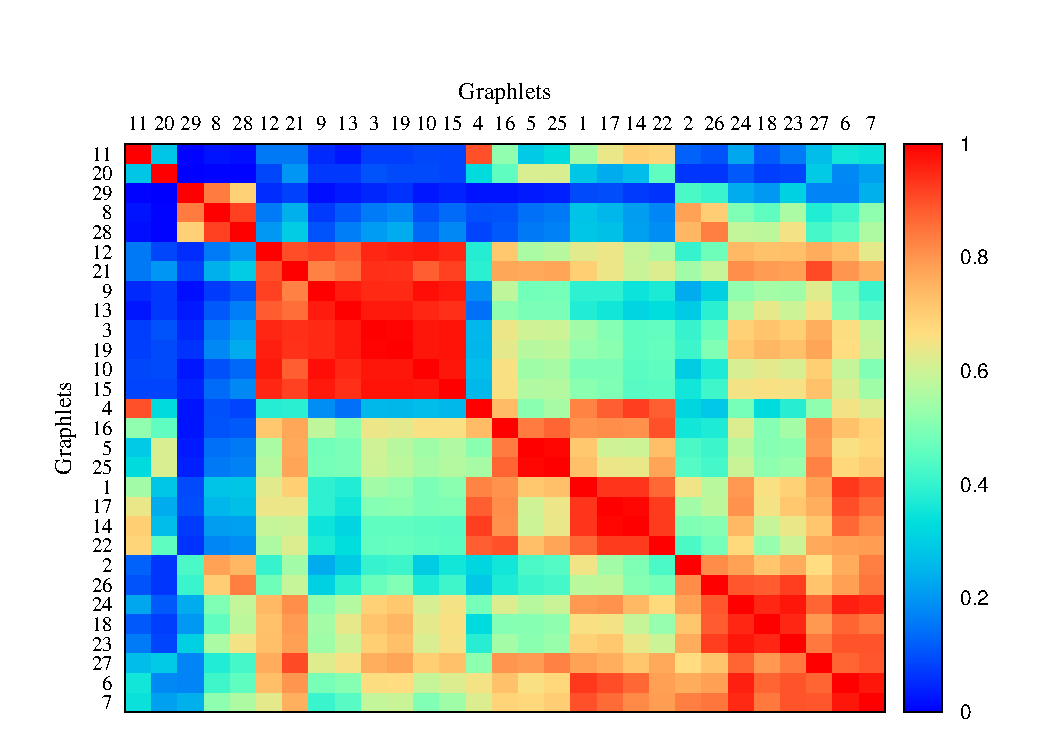
\includegraphics[scale=1.0]{../code/final_results/hsa_metabolic_network/heatmap_pearsons_hclust_hsa_metabolic_network-poly-32.pdf}}
  \caption[Pearson's GCV correlation matrix heat map for the compound-based Human Metabolic network.]{Pearson's GCV correlation matrix heat map for the compound-based Human Metabolic network. The heat map has been normalised with feature scaling and a $3^{rd}$ degree polynomial and hierarchically clustered.}
  \label{meta_heatmap_hclust_3}
\end{figure}

 
Furthermore, we notice that graphlets from clusters $A$,$B$ and $C$ also have a certain amount of inter-correlation between them, with inter-correlation values of at least 0.5. However, this is not the case for cluster $D$, which is made of cliques. The cliques only bear some correlation with cluster $C$ made of triangle-like graphlets, which is not surprising for the following reasons:
\begin{itemize}
 \item Cliques contain a lot of triangles
 \item Cliques do not contain claws $C_n$ or paths $P_n$, which miss several edges.
\end{itemize}

It should also be noted that graphlets $G_{11}$ and $G_{20}$ have been left outside, as they don't strongly correlate with any of the other groups. The cluster closest to these 2 graphlets is the claw cluster. To sum up, we conclude that graphlets cluster together according to what basic shapes they contain.

\subsection{Canonical Correlation Analysis}

In order to run Canonical Correlation Analysis on the metabolic networks we used \emph{Enzyme Commission} (EC) numbers as annotations for the network nodes. More information about EC numbers can be found in background section \ref{metabolic_annotations}. Basically, EC numbers are used to annotate each enzyme in the metabolic network according to the type of reaction it catalyses. The results of the CCA analysis using EC numbers is presented in figure \ref{hsa_metabolic_network_cca}.

\begin{figure}
  \begin{subfigure}{.65\textwidth}
  \centering
  \begin{tabular}{ c c | c c }
    \multicolumn{2}{c}{Canonical Correlation} &  \multicolumn{2}{c}{0.51769} \\
    \multicolumn{2}{c}{p-value} &  \multicolumn{2}{c}{0.00000} \\
    \hline
    \multicolumn{2}{c}{X variate} & \multicolumn{2}{c}{Y variate}\\
    \hline
  EC5 & -0.11422 &  G20 & -0.13839\\
  EC2 & -0.12601 &  G11 & -0.17646\\
  EC4 & -0.16144 &  G9 & -0.17733\\
  EC1 & -0.16156 &  G10 & -0.18420\\
  EC3 & -0.21057 &  G13 & -0.18757\\
  EC6 & -0.40615 &  G16 & -0.20243\\
  & &  G12 & -0.20399\\
  & &  G4 & -0.20521\\
  & &  G15 & -0.20553\\
  & &  G3 & -0.20671\\
  & &  G19 & -0.20956\\
  & &  G22 & -0.21329\\
  & &  G5 & -0.21897\\
  & &  G25 & -0.22033\\
  & &  G14 & -0.22256\\
  & &  G17 & -0.23125\\
  & &  G21 & -0.23144\\
  & &  G18 & -0.24860\\
  & &  G1 & -0.25408\\
  & &  G27 & -0.25641\\
  & &  G6 & -0.26110\\
  & &  G24 & -0.26365\\
  & &  G23 & -0.26813\\
  & &  G7 & -0.28239\\
  & &  G26 & -0.28362\\
  & &  G28 & -0.32754\\
  & &  G29 & -0.34583\\
  & &  G2 & -0.36785\\
  & &  G8 & -0.37442\\
  \end{tabular}

  \end{subfigure}
  \begin{subfigure}{.25\textwidth}
    \centering 
    \rowcolors{1}{}{}		
	
    \gtwenty
    \geleven
    \gnine
    \gdots
    \gtwentynine
    \gtwo
    \geight

  \end{subfigure}
  
\caption[CCA analysis on the compound-based Human Metabolic network.]{CCA analysis on the compound-based Human Metabolic network. The CCA is 0.51, with a p-value smaller than 0.0001. We notice that all EC numbers correlate positively with all the graphlets because their cross-loadings have the same sign. In the $X$ variate EC6 shows the highest correlation while in the $Y$ variate cliques \{8,2,29\} show the highest correlation. Note that the p-value is not exactly zero, but it was truncated to zero because of floating point approximations.}
\label{hsa_metabolic_network_cca}
\end{figure}

There is some degree of correlation between the Graphlets and the EC numbers ($\rho = 0.517 $), with a p-value smaller than 0.05. All the cross-loadings from both the graphlets and the EC numbers have the same sign, which suggests that they are positively correlated. Cliques \{8,2,29\} have the highest magnitude in their weights, while EC6 (ligands) have the highest magnitude in the EC vector. 

EC6 refers to Ligases, which are enzymes that can catalyse the joining of two large molecules by forming a new chemical bond. The reason why the magnitude of EC6 is quite high (0.4) compared to the other indicators is because the two large molecules catalysed by EC6 enzymes are represented in the metabolic network by cliques or dense clusters which have a lot of interactions and feedback loops between them. This is why cliques \{8,2,29\} or dense graphlets such as $G_{28}$ have the cross-loadings with the highest magnitude. However, this doesn't exclude other sparser protein groups to be part of the two molecules catalysed by the Ligase, since graphlets such as \{9,10,11 or 12\} also correlate positively with EC6. Regarding the other functional groups, we cannot say much about them because the magnitude of their cross-loading is relatively smaller compared to the cross-loading of EC6. 


\subsection{CCA Results for other model organisms}

We have analysed other compound-based metabolic networks that belong to the following organisms: C. elegans, D.melanogaster, E.coli, M.musculus, S.cerevisiae. These experiments confirm the results obtained for the human metabolic network. Average CCA correlation is around 0.5, EC6 has the highest magnitude at around 0.4 and cliques \{2,8,29\} are the graphlets most correlated with EC6 ($\rho = 0.35$).

The same methodology has also been applied to enzyme-based metabolic networks for all the 6 different organisms. However, these display a much lower CCA correlation (around 0.25), having p-values that are above 0.05, suggesting that the results are not statistically significant. This is the case for all the organisms, including humans. The graphlet signatures have very low signatures, while EC numbers don't have magnitudes above 0.22. These results have not been included in the report, but are available in the source code, under the \lstinline|code/final_results/| folder\footnote{The relevant folders are: \lstinline|hsa_meta_ec_omer|, \lstinline|cel_metabolic|, \lstinline|dme_metabolic|, \lstinline|eco_metabolic|, \lstinline|mmu_metabolic|, \lstinline|sce_metabolic|, }.

\subsection{CCA on the KEGG categories}

We have also tried to use the KEGG categories as annotations for the enzymes in the metabolic network. We have initially annotated the enzymes with the following high-level categories:
\begin{itemize}
 \item Metabolism
 \item Genetic Information Processing
 \item Environmental Information Processing
 \item Cellular Processes
 \item Organismal Systems
 \item Human Diseases
\end{itemize}

The CCA correlation obtained was only around 0.6, so we tried running CCA on the lower-level categories. That is, for each of those 6 high-level categories, we ran CCA on its subcategories. The best results were obtained for Human Diseases, Cellular Processes and Organismal Systems and are presented in the following subsections.

\subsection{Cellular Processes}
\label{cca_kegg_cellular}

The overall CCA correlation for Cellular Processes is 0.98, which is quite high compared to previous CCAs, and the p-value is smaller than 0.00001.  Figure \ref{cellular_cca} shows the CCA for Cellular Processes. We observe that graphlet $G_9$ correlates positively with \emph{Transport and Catabolism}. The reason for this is because in Catabolism, large molecules such as polysaccharides, lipids and nucleic acids are broken down into smaller units such as monosaccharides, fatty acids or nucleotides. Since molecules such as polysaccharides are made up of long chains of small monomer units, graphlets that are made of long paths such as $G_9$ will be overly represented in these processes. Similarly, enzymes involved in transport are transporting nutrients from one chemical to another, so their interactions will be characterised by long "transportation" paths that are best represented by graphlet $G_9$. 
At the other end of the spectrum, \emph{Cell growth and death} and \emph{Cell communication} are correlated with graphlets \{1,2,7,8\}. The reason for this is because in Cell Communication, if a cell is stimulated, it's needs to send signals to its neighbours through the use of molecules. First of all, in order to ensure that a signal is successfully transmitted, several molecules carrying the same message could be transmitted and there must be different possible paths to reach the destination. If this is not the case, then the message will get lost when the path is disrupted or the messenger molecule stops functioning. This is why a graphlet like $G_9$ correlates negatively with these, because $G_9$ is made of a long path of 5 nodes and if one of the nodes fails, then the whole signal is lost. Graphlets \{2,7,8\} correlate positively because these are highly connected (\{2,8\} are cliques) or because they contain several alternative paths for message transmission ($G_7$). However, the reason why graphlet $G_
1$ correlates with Cell Communication is still a matter or research.


\begin{figure}
  \begin{subfigure}{.65\textwidth}
  \centering
  \textbf{Cellular Processes CCA}\par\medskip
  \begin{tabular}{ c c | c c }
    \multicolumn{2}{c}{Canonical Correlation} &  \multicolumn{2}{c}{0.98633} \\
    \multicolumn{2}{c}{p-value} &  \multicolumn{2}{c}{0.00000} \\
    \hline
    \multicolumn{2}{c}{X variate} & \multicolumn{2}{c}{Y variate}\\
    \hline
  Transport and catabolism & 0.52121 &  G9 & 0.04828\\
  Cell motility & 0.20502 &  G21 & 0.01960\\
  Cell communication & -0.40751 &  G25 & 0.01441\\
  Cell growth and death & -0.69712 &  G5 & 0.01434\\
  & &  G16 & 0.00969\\
  & &  G13 & 0.00199\\
  & &  G12 & -0.00048\\
  & &  G27 & -0.00134\\
  & &  G20 & -0.00256\\
  & &  G3 & -0.00412\\
  & &  G24 & -0.01287\\
  & &  G19 & -0.01528\\
  & &  G10 & -0.01623\\
  & &  G18 & -0.01681\\
  & &  G14 & -0.02579\\
  & &  G11 & -0.02667\\
  & &  G23 & -0.02851\\
  & &  G15 & -0.03092\\
  & &  G17 & -0.03201\\
  & &  G29 & -0.04271\\
  & &  G6 & -0.04386\\
  & &  G28 & -0.04750\\
  & &  G4 & -0.05059\\
  & &  G26 & -0.05235\\
  & &  G22 & -0.05877\\
  & &  G8 & -0.05881\\
  & &  G7 & -0.07069\\
  & &  G2 & -0.07388\\
  & &  G1 & -0.07463\\
  \end{tabular}

  \end{subfigure}
  \begin{subfigure}{.25\textwidth}
    \centering 
    \rowcolors{1}{}{}		
	
    \gnine
    \gtwentyone
    \gtwentyfive
    \gdots
    \gseven
    \gtwo
    \gone

  \end{subfigure}
  
\caption[CCA on the Human Metabolic network using Cellular Processes from KEGG]{CCA on the Human Metabolic network using Cellular Processes from KEGG. The correlation value is high ($\rho = 0.98$) and the p-value is smaller than 0.00001, suggesting a very strong correlation. Transport and catabolism and cell motility correlate with the upper part of the graphlet spectrum: \{9,21,25,5, \dots\} because their cross-loadings have the same sign. Similarly, Cell Communication and Cell growth and death correlate with the lower end of the graphlet spectrum: \{1,2,7,8, \dots\}. }
\label{cellular_cca}
\end{figure}



\subsection{Organismal Systems}
\label{cca_kegg_organismal}

Figure \ref{organismal_cca} shows the CCA for \emph{Organismal Systems}. The CCA correlation is also very high (0.96) and the p-value smaller than 0.0001. These cross-loadings suggest that enzymes involved in Environmental Adaptation and Excretory systems are usually rich in interactions and their neighbours are also highly clustered, since all the graphlets correlate positively with these systems. On the other hand, enzymes involved in Circulatory and Digestive metabolic pathways have sparse  neighbourhoods that would ideally contain few graphlets. One explanation for this is because in these systems enzymes, proteins and metabolites have to circulate throughout the whole body and interact with distant enzymes, which don't cluster together. Enzymes at the other end of the spectrum (Environmental Adaptation and Excretory system) are much more localised in the body. For instance, excretory system enzymes are mainly active in the kidney or liver. Moreover, the enzymes involved in the Circulatory and Digestive 
systems will probably have less interactions compared to their counterparts in the Environmental Adaptation and Excretory systems, because a neighbourhood sparse in graphlets is usually an indication of it being small.



\begin{figure}
  \centering
  \textbf{Organismal Systems CCA}\par\medskip
  \begin{subfigure}{.65\textwidth}
  \centering
  \begin{tabular}{ c c | c c }
    \multicolumn{2}{c}{Canonical Correlation} &  \multicolumn{2}{c}{0.96925} \\
    \multicolumn{2}{c}{p-value} &  \multicolumn{2}{c}{0.00000} \\
    \hline
    \multicolumn{2}{c}{X variate} & \multicolumn{2}{c}{Y variate}\\
    \hline
  Environmental adaptation & 0.20426 &  G26 & 0.30978\\
  Excretory system & 0.19729 &  G24 & 0.29818\\
  Development & 0.07461 &  G23 & 0.29308\\
  Endocrine system & 0.04192 &  G18 & 0.28901\\
  Nervous system & -0.01315 &  G6 & 0.27857\\
  Sensory system & -0.06276 &  G12 & 0.26520\\
  Immune system & -0.15192 &  G19 & 0.25419\\
  Digestive system & -0.23211 &  G3 & 0.24988\\
  Circulatory system & -0.37659 &  G14 & 0.23274\\
  & &  G13 & 0.23155\\
  & &  G1 & 0.22611\\
  & &  G17 & 0.22546\\
  & &  G7 & 0.21225\\
  & &  G27 & 0.20440\\
  & &  G10 & 0.19976\\
  & &  G9 & 0.19547\\
  & &  G25 & 0.19422\\
  & &  G16 & 0.19135\\
  & &  G28 & 0.18874\\
  & &  G4 & 0.18421\\
  & &  G5 & 0.18381\\
  & &  G20 & 0.17359\\
  & &  G11 & 0.15537\\
  & &  G21 & 0.14453\\
  & &  G29 & 0.11208\\
  & &  G8 & 0.10681\\
  & &  G2 & 0.10369\\
  & &  G22 & 0.08192\\
  & &  G15 & 0.01276\\
  \end{tabular}

  \end{subfigure}
  \begin{subfigure}{.25\textwidth}
    \centering 
    \rowcolors{1}{}{}		
	
    \gtwentysix
    \gtwentyfour
    \gtwentythree
    \gdots
    \gtwo
    \gtwentytwo
    \gfifteen

  \end{subfigure}
  
\caption[CCA on the Human Metabolic network between different Organismal Systems and the GCV signature of enzymes.]{CCA on the Human Metabolic network between different Organismal Systems and the GCV signature of enzymes. The correlation value is again high ($\rho = 0.96$) and the p-value is small ($p < 0.00001$). Environmental adaptation, Excretory system, Development and the Endocrine system correlate positively with all the graphlets, while the Circulatory, Digestive, Immune, Sensory and Nervous systems correlate negatively. The actual p-value is not exactly zero but it is shown as zero because of floating point approximations.}
\label{organismal_cca}
\end{figure}




\subsection{Human Diseases}
\label{cca_kegg_human}

Figure \ref{fig:metabolic_diseases_cca} shows the CCA for various Human Diseases such as Cancers, Immune diseases, Neurodegenerative diseases or Cardiovascular diseases. The result that is most striking here is that Cardiovascular diseases and Substance dependence correlate negatively with almost all the graphlets (apart from \{2,8\}). This implies that the enzymes and proteins involved in these Human Diseases have a low number of interactions and when they do have interactions, their neighbourhood only contains small clusters of 3--4 nodes maximum. The explanation for this might be the same as for the Organismal Systems: the enzymes involved in Cardiovascular diseases and Substance dependence travel across long pathways throughout the body and end up interacting with distant chemicals that do not interact with each other because of their distant location in the body. However, the small clusters of interactions might occur because of locality, that is all chemicals involved will be in the same area and 
therefore inevitably interact with each other. In the case of the Cardiovascular diseases, the enzymes travel long distances because they are transported through the blood vessels, while the ones involved in Substance dependence are again transported through the blood vessels or other channels. We cannot say anything about the rest of the diseases (Cancers, Immune Diseases, etc \dots) because their relative cross-loadings have a very low magnitude relative to the others.


\begin{figure}
  \centering
  \textbf{Human Diseases CCA}\par\medskip
  \begin{subfigure}{.65\textwidth}
  \centering
  \begin{tabular}{ c c | c c }
    \multicolumn{2}{c}{Canonical Correlation} &  \multicolumn{2}{c}{0.99479} \\
    \multicolumn{2}{c}{p-value} &  \multicolumn{2}{c}{0.00000} \\
    \hline
    \multicolumn{2}{c}{X variate} & \multicolumn{2}{c}{Y variate}\\
    \hline
  Cardiovascular diseases & 0.99171 &  G2 & 0.01681\\
  Substance dependence & 0.57989 &  G8 & 0.00462\\
  Infectious diseases & 0.21844 &  G29 & -0.00737\\
  Neurodegenerative diseases & 0.00366 &  G7 & -0.00812\\
  Endocrine and metabolic diseases & -0.02545 &  G1 & -0.00989\\
  Immune diseases & -0.03029 &  G26 & -0.01077\\
  Cancers & -0.08682 &  G24 & -0.01274\\
  & &  G6 & -0.01321\\
  & &  G28 & -0.01321\\
  & &  G15 & -0.01342\\
  & &  G23 & -0.01369\\
  & &  G22 & -0.01420\\
  & &  G21 & -0.01438\\
  & &  G14 & -0.01449\\
  & &  G12 & -0.01465\\
  & &  G17 & -0.01516\\
  & &  G16 & -0.01521\\
  & &  G18 & -0.01526\\
  & &  G13 & -0.01528\\
  & &  G19 & -0.01562\\
  & &  G9 & -0.01565\\
  & &  G10 & -0.01641\\
  & &  G4 & -0.01727\\
  & &  G3 & -0.01742\\
  & &  G11 & -0.01781\\
  & &  G20 & -0.01936\\
  & &  G25 & -0.02017\\
  & &  G5 & -0.02438\\
  & &  G27 & -0.02731\\
  \end{tabular}


  \end{subfigure}
  \begin{subfigure}{.25\textwidth}
    \centering 
    \rowcolors{1}{}{}		
	
    \gtwo
    \geight
    \gtwentynine
    \gdots
    \gtwentyfive
    \gfive
    \gtwentyseven

  \end{subfigure}
  
\caption[CCA Analysis on the Human Metabolic network between Human Diseases and the GCV signature.]{CCA Analysis on the Human Metabolic network between Human Diseases and the GCV signature. The correlation value is high ($\rho = 0.96$) while the p-value is very small ($p < 0.00001$). The actual p-value outputted by the program is 0.0 due to floating-point approximations. Cardiovascular diseases, Substance dependence, Infectious and Neurodegenerative diseases correlate positively with all the graphlets, while the Endocrine and Metabolic diseases, Immune diseases and Cancers correlate negatively.}
\label{fig:metabolic_diseases_cca}
\end{figure}




